%%%%%%%%%%%%%%%%%%%%%%%%%%%%%%%%%%%%%%%%%%%%%%%%%%%%%%%%%%%%%%%%%%%%%%%%%%%%
% AGUJournalTemplate.tex: this template file is for articles formatted with LaTeX
%
% This file includes commands and instructions
% given in the order necessary to produce a final output that will
% satisfy AGU requirements, including customized APA reference formatting.
%
% You may copy this file and give it your
% article name, and enter your text.
%
% guidelines and troubleshooting are here: 

%% To submit your paper:
\documentclass[draft]{agujournal2019}
\usepackage{url} %this package should fix any errors with URLs in refs.
\usepackage{lineno}
\usepackage[inline]{trackchanges} %for better track changes. finalnew option will compile document with changes incorporated.
\usepackage{soul}
\linenumbers
%%%%%%%
% As of 2018 we recommend use of the TrackChanges package to mark revisions.
% The trackchanges package adds five new LaTeX commands:
%
%  \note[editor]{The note}
%  \annote[editor]{Text to annotate}{The note}
%  \add[editor]{Text to add}
%  \remove[editor]{Text to remove}
%  \change[editor]{Text to remove}{Text to add}
%
% complete documentation is here: http://trackchanges.sourceforge.net/
%%%%%%%

\draftfalse

%% Enter journal name below.
%% Choose from this list of Journals:
%
% JGR: Atmospheres
% JGR: Biogeosciences
% JGR: Earth Surface
% JGR: Oceans
% JGR: Planets
% JGR: Solid Earth
% JGR: Space Physics
% Global Biogeochemical Cycles
% Geophysical Research Letters
% Paleoceanography and Paleoclimatology
% Radio Science
% Reviews of Geophysics
% Tectonics
% Space Weather
% Water Resources Research
% Geochemistry, Geophysics, Geosystems
% Journal of Advances in Modeling Earth Systems (JAMES)
% Earth's Future
% Earth and Space Science
% Geohealth
%
% ie, \journalname{Water Resources Research}

\journalname{JGR: Atmospheres}


\begin{document}

%%%%%%%%%%%%%%%%%%%%%%%%%%%%%%%%%%%%%%%%%%%%%%%
%  TITLE
%
% (A title should be specific, informative, and brief. Use
% abbreviations only if they are defined in the abstract. Titles that
% start with general keywords then specific terms are optimized in
% searches)
%
%%%%%%%%%%%%%%%%%%%%%%%%%%%%%%%%%%%%%%%%%%%%%%%

% Example: \title{This is a test title}

\title{Inland-Penetrating Atmospheric Rivers and Hydrometeorological Impacts in Colorado}

%%%%%%%%%%%%%%%%%%%%%%%%%%%%%%%%%%%%%%%%%%%%%%%
%
%  AUTHORS AND AFFILIATIONS
%
%%%%%%%%%%%%%%%%%%%%%%%%%%%%%%%%%%%%%%%%%%%%%%%

% Authors are individuals who have significantly contributed to the
% research and preparation of the article. Group authors are allowed, if
% each author in the group is separately identified in an appendix.)

% List authors by first name or initial followed by last name and
% separated by commas. Use \affil{} to number affiliations, and
% \thanks{} for author notes.
% Additional author notes should be indicated with \thanks{} (for
% example, for current addresses).

% Example: \authors{A. B. Author\affil{1}\thanks{Current address, Antartica}, B. C. Author\affil{2,3}, and D. E.
% Author\affil{3,4}\thanks{Also funded by Monsanto.}}

% \authors{=list all authors here=}

\authors{Deanna Nash\affil{1}, Jonathan J. Rutz\affil{1}, Jason Cordeira \affil{1}, F. Martin Ralph \affil{1}, Kris Sanders \affil{2}, Erin Walter \affil{2}}


% \affiliation{1}{First Affiliation}
% \affiliation{2}{Second Affiliation}
% \affiliation{3}{Third Affiliation}
% \affiliation{4}{Fourth Affiliation}

% \affiliation{=number=}{=Affiliation Address=}
\affiliation{1}{Center for Western Weather and Water Extremes, Scripps Institute of Oceanography, University of California San Diego, California}
\affiliation{2}{National Weather Service, Weather Forecast Office, Grand Junction, Colorado}
%(repeat as many times as is necessary)


% Corresponding author mailing address and e-mail address:

% (include name and email addresses of the corresponding author.  More
% than one corresponding author is allowed in this LaTeX file and for
% publication; but only one corresponding author is allowed in our
% editorial system.)

% Example: \correspondingauthor{First and Last Name}{email@address.edu}

\correspondingauthor{Deanna Nash}{dnash@ucsd.edu}



%%%%%%%%%%%%%%%%%%%%%%%%%%%%%%%%%%%%%%%%%%%%%%%
% KEY POINTS
%%%%%%%%%%%%%%%%%%%%%%%%%%%%%%%%%%%%%%%%%%%%%%%
%  List up to three key points (at least one is required)
%  Key Points summarize the main points and conclusions of the article
%  Each must be 140 characters or fewer with no special characters or punctuation and must be complete sentences

% Example:
% \begin{keypoints}
% \item	List up to three key points (at least one is required)
% \item	Key Points summarize the main points and conclusions of the article
% \item	Each must be 140 characters or fewer with no special characters or punctuation and must be complete sentences
% \end{keypoints}

\begin{keypoints}
\item enter point 1 here
\item enter point 2 here
\item enter point 3 here
\end{keypoints}

%%%%%%%%%%%%%%%%%%%%%%%%%%%%%%%%%%%%%%%%%%%%%%%
%
%  ABSTRACT and PLAIN LANGUAGE SUMMARY
%
% A good Abstract will begin with a short description of the problem
% being addressed, briefly describe the new data or analyses, then
% briefly states the main conclusion(s) and how they are supported and
% uncertainties.

% The Plain Language Summary should be written for a broad audience,
% including journalists and the science-interested public, that will not have 
% a background in your field.
%
% A Plain Language Summary is required in GRL, JGR: Planets, JGR: Biogeosciences,
% JGR: Oceans, G-Cubed, Reviews of Geophysics, and JAMES.
% see http://sharingscience.agu.org/creating-plain-language-summary/)
%
%%%%%%%%%%%%%%%%%%%%%%%%%%%%%%%%%%%%%%%%%%%%%%%

%% \begin{abstract} starts the second page

\begin{abstract}
Atmospheric rivers (ARs) play a leading role in high-impact weather and long-term hydroclimate across the Western U.S., being both the primary drivers of flood damage and major contributors to water supply across much of this region. In response, the community has developed an extensive knowledge of AR frequency, intensity, impacts, key meteorological processes, and predictive skill, but this knowledge is primarily focused on ARs at or near landfall on the U.S. West Coast. Relatively little work has been done to understand AR characteristics further inland and this is especially true for Colorado, where high and complex topography, as well as distance from the coast, frustrate attempts to track ARs, AR-derived moisture, and AR-related impacts. While a large volume of anecdotal evidence suggests that ARs play a fundamental role in extreme precipitation and longer-term hydroclimate across Colorado, this relationship is yet to be systematically analyzed and quantified. This work uses novel methods to explore the role of ARs, their landfalling intensity, and their interannual variability on hydrometeorological extremes and impacts across the state, focusing on the relative contribution of inland-penetrating ARs to top-decile precipitation. 

We show that while the overhead AR frequency across Colorado is very low, moisture sourced from landfalling ARs affects this area much more frequently, penetrating inland along relatively low-elevation corridors through the Interior West. Consequently, AR contributions to precipitation across Colorado are higher than previous studies suggest, and exhibit substantial geographic and interannual variability. In addition, we highlight new forecast tools that enable better prediction of these events, developed in collaboration with National Weather Service offices across the state. 

\end{abstract}

\section*{Plain Language Summary}
Enter your Plain Language Summary here or delete this section.
Here are instructions on writing a Plain Language Summary: 
https://www.agu.org/Share-and-Advocate/Share/Community/Plain-language-summary


%%%%%%%%%%%%%%%%%%%%%%%%%%%%%%%%%%%%%%%%%%%%%%%
%
%  BODY TEXT
%
%%%%%%%%%%%%%%%%%%%%%%%%%%%%%%%%%%%%%%%%%%%%%%%

%%% Suggested section heads:
\section{Introduction}
\label{intro}

In Colorado, forecasting precipitation is challenging due to its high spatio-temporal variability \cite{Serreze2001CharacteristicsData, Cowie1986ColoradoAnalysis, Kirk2018LargeBasin, Lute2014RoleStates}. In the western region of Colorado in the slopes of the Rocky Mountains, a majority of the total annual precipitation falls during the winter months between November and February \cite{Doesken1984Period., Harvey2019CitizensFrom}. In southeastern Colorado, along the Front Range and in the Plains, most of the precipitation falls during the summer months during convective storms, while a majority of the precipitation in northeastern Colorado falls during the spring months \cite{Doesken1984Period., Harvey2019CitizensFrom}. Even during the same storm, there is large variation in precipitation across short distances due to high and complex topography in Colorado. \citeA{Serreze2001CharacteristicsData} found that on the western slopes of Colorado, less than 50\% of the time a heavy or extreme precipitation event occurs at one station, most of the other surrounding stations also experience a heavy precipitation event. Furthermore, single storm events can contribute significantly to total water year precipitation, as demonstrated by \citeA{Serreze2001CharacteristicsData, Cowie1986ColoradoAnalysis, Kirk2018LargeBasin, Lute2014RoleStates}.

% "Serreze et al.'s 2001 analysis of large snowfall events in the Western United States found that the largest snowfall event of each year contributed 10–23% of the annual snow water equivalent (SFE) at SNOTEL stations."

One type of storm that results in heavy precipitation across the western U.S. is an atmospheric river (AR). ARs are defined as long, but narrow bands of intense water vapor transport, that when crossing from ocean to land or interacting with complex topography, may result in heavy precipitation \cite<e.g.,>[and others]{dettinger2016historical, Newell1994, Newell1992, Ralph2012}. While many studies show that ARs modulate extreme precipitation in multiple regions across the globe, there are few studies that demonstrate the high contribution to extreme and annual precipitation from ARs that penetrate inland and travel long distances \cite{Rutz2012, Rutz2014, Rutz2015, Nash2021, Nash2024InfluenceExtremes}. In particular, \citeA{Rutz2012} found that up to 20\% of cool-season (November to April) precipitation at SNOTEL stations occurred within a day of an AR crossing the U.S. West Coast between the latitudes of 24\textdegree N and 52.5\textdegree N. \cite{Rutz2014} found that ARs occur directly over Colorado less than 5\% of the time (during cool-season months between 1988 and 2011) and contribute up to 15\% of cool season precipitation. While the AR identification method in \citeA{Rutz2014} uses an absolute threshold for IVT (IVT $>$ 250 kg m\textsuperscript{-1} s\textsuperscript{-1}), other AR detection tools that use percentile based thresholds (e.g., \citeA{Guan2015}, IVT $>$ 85th percentile) show similar results over western Colorado, where ARs occur less than 8\% of the time, and contribute 15--20\% of cool season precipitation. 

However, there is anecdotal evidence from forecasters at the National Weather Service Forecast Offices in Grand Junction, CO that moisture from ARs reaches Colorado more frequently than previously thought, and are contributing significantly to precipitation in Colorado, particularly heavy or extreme precipitation events. This study aims to quantify the contribution of AR moisture to precipitation in Colorado, but rather than rely on detecting an AR overhead, we use backwards trajectory analysis to show there is a much higher frequency of AR related moisture penetrating inland and triggering a precipitation response in Colorado. \citeA{Rutz2015} used forward trajectory analysis to analyze the common pathways and characteristics of cool-season ARs that made landfall on the U.S. West Coast and penetrated inland. They found that the highest frequency of ARs that are able to penetrate inland make landfall north of 45\textdegree N along the U.S. West Coast, and follow low-elevation cooridoors inland. They also found that although a smaller number of ARs make landfall on the Baja Peninsula, they have a higher success rate (52\% of the time) of penetrating inland compared to those that make landfall at higher latitudes (24--28\% of the time) \cite{Rutz2015}. However, this study did not attribute fraction of precipitation in interior west locations associated with these tracked ARs, and furthermore, very few of the trajectories extended past 110\textdegree W. \citeA{Alexander2015} used backwards trajectory analysis to identify dominant moisture pathways during cool-season extreme precipitation events in the Intermountain West, and found similar results to those of \citeA{Rutz2015}, but did not directly attribute precipitation to ARs. 

To address these caveats, we combine the approaches of \citeA{Rutz2015, Alexander2015} to attribute moisture from coastal landfalling ARs to top-decile ($>$ 90th percentile) precipitation across Colorado. We employ backwards trajectories from the top-decile precipitation days in all the subbasins in Colorado, and determine if precipitation from a particular day was associated with a coastal AR, as well as determine the likely pathways of the AR-related moisture transport. We show that there is higher frequency of AR-related moisture penetrating inland and contributing to top-decile precipitation days than previously found. The organization of this paper is as follows: Section \ref{sec:data} describes the data used in this analysis and Section \ref{sec:methods} outlines the methodology used for the backwards trajectory analysis. Section \ref{sec:results:contribution} quantifies the contribution of AR-related moisture to top-decile precipitation days across Colorado and Section \ref{sec:results:moisture_pathways} describes the moisture pathways of the AR-related precipitation days. Results, applications, and future directions are summarized in Section \ref{conclusions}. 

% Main Idea: When you identify ARs over Colorado using traditional ARDTs and considering the days when an AR is directly overhead, you get very few ARs per year (less than 1 per year); therefore the goal of this paper is to objectively identify moisture from ARs that is penetrating inland, reaching Colorado, and triggering a precipitation response. *** Present this as an existing paradox that needs explanation ***
% Introduce: Can reference studies (Rutz et al., 2014; Guan and Waliser, 2015; Guan and Waliser, 2022  (AR Scale/ARDT)) that show the frequency of ARs overhead in Colorado as very few. 
% Key Point: Describe the use of trajectory analysis and it’s benefits in tracking air parcels associated with precipitation (Find some more studies, but can reference the Alexander et al., 2018 paper) 
% Explain Key Point: This point needs to be made now because it sets up why we did what we did for our methods
% Connect: This key point connects to the main point because we can now show that there are actually a much higher frequency of AR related moisture penetrating inland and triggering precipitation response. This has implications for weather forecasting (potential avenue to improve short term forecasting) as well as longer term hydroclimate implications (number of ARs per year influencing drought conditions)

% Motivation
% Quantify the precipitation contribution of AR moisture that reach CO
% Develop a methodology for attributing precipitation over the Western U.S. Interior to landfalling ARs along the U.S. West Coast and Gulf Coast and apply it to CO knowing that ARs break up and don’t meet traditional criteria by the time they reach CO

% Develop specialized AR-focused diagnostic and forecasting tools for the Colorado Front Range 
% Develop a tool and show it in use - for a single event




\section{Data}
\label{sec:data}
\subsection{Colorado Watershed Boundaries}
To determine the contribution of AR related moisture to extreme precipitation days in Colorado, we use the Watershed Boundary Dataset created by the U.S. Geological Survey, U.S. Department of Agriculture - Natural Resource Conservation Service (NRCS), and U.S. Environmental Protection Agency. The polygon-based dataset represents the hydrologic unit (HU) boundaries to the 8-digit (HUC8) and identifies 92 HUC8 subbasins (hereafter referred to as subbasins) that touch Colorado. Additionally, we show analysis at the region level, which indicates that results for all subbasins (of the 92 analyzed) that share the first two digits of their HU code. For example, we summarize results for Colorado subbasins that fall within the Rio Grande Region (HUC2 13), which shows the results for the xx subbasins whose first two digits of the HUC8 of are 13 (Colorado Region HUC2 is 14, South Platte Region HUC2 is 10, and Arkansas Region HUC2 is 11).

\subsection{Reanalysis Data}

The European Centre for Medium-Range Weather Forecasts (ECMWF) atmospheric reanalyses of the global climate (ERA5) at 1-h and  0.25\textdegree{} resolutions were used to examine geopotential height, winds, specific humidity at multiple pressure levels, as well as IVT \cite{Hersbach2020}. Zonal and meridional IVT were calculated by taking the 1-hourly reanalyses, interpolating u and v wind components (m s\textsuperscript{-1}), and water vapor mixing ratio (kg kg\textsuperscript{-1}) between 300 hPa and the surface (see Appendix \ref{appendix:ivt} for equations). The vertical fluxes of water vapor were calculated by multiplying the v (meridional) or u (zonal) component wind by specific humidity (q) at each pressure level (see Appendix \ref{appendix:wvf} for equations).

\subsection{Precipitation Data}

For precipitation, we generated daily time series for each subbasin based on daily total precipitation (rain and melted snow) provided by the Parameter-elevation Regressions on Independent Slopes Model (PRISM). The daily total precipitation is area aggregated to the HUC8 subbasins from 1 Jan 2000 to 31 Dec 2023 where the 24-hour precipitation ends at 12 UTC of each day. Mean areal precipitation is calculated by identifying the latitude and longitude pairs on a 0.05\textdegree{} grid that fall in each subbasin and using bilinear interpolation to interpolate the PRISM 4-km grid to those points within the subbasin. The point values are then averaged within each subbasin, giving mean areal precipitation in mm per day. 

%% which PRISM dataset did Jay download? https://prism.oregonstate.edu/documents/PRISM_datasets.pdf

We used the distribution of precipitation values for each subbasin to determine the 90th percentile threshold, only considering days when precipitation is greater than 2.54 mm (0.1 inch). We ran trajectories for all days in each subbasin where precipitation exceeded 90th percentile, hereafter referred to as top-decile precipitation days.


\subsection{AR Detection}

Three commonly used AR detection tools (ARDTs) were employed to detect ARs: (1) the Tracking Atmospheric Rivers Globally as Elongated Targets (tARget) algorithm version 4 was applied to global, 1-h, 0.25\textdegree{} horizontal resolution ERA5 from 1940 to 2023 \cite{Guan2024AERA5}. The tARget v4 uses a combination of geometry (e.g., length, width), relative IVT intensity thresholds (e.g., above 85th percentile of local climatological IVT), and directional components (e.g., must be poleward) to detect AR objects. Additionally, tARget v4 is a combination of condition (meeting the threshold and geometry requirements) and tracking (AR object is followed across time and space) computation type. (2) the \citeA{Rutz2014} method was applied to global, 3-h, 0.5\textdegree{}x0.625\textdegree{} horizontal resolution Modern Era Retrospective Reanalysis Version 2 (MERRA2) from 1980 to 2023 (hereafter referred to as the Rutz ARDT) \cite{Bosilovich2015, Gelaro2017}. The Rutz ARDT uses a combination of geometry and absolute IVT intensity thresholds (e.g. greater than or equal to 250 kg m-1 s-1). (3) the AR Scale \cite{MartinRalph2019} was applied to global, 1-h, 0.25\textdegree{} horizontal resolution ERA5 from 2000 to 2023. The AR Scale identifies ARs using a point-based value of 1--5 based on the maximum IVT magnitude and the duration of IVT $>$ 250 kg m\textsuperscript{-1} s\textsuperscript{-1} at that point \cite{MartinRalph2019}. Points must sustain IVT $>$ 250 kg m\textsuperscript{-1} s\textsuperscript{-1} for at least 24 hours to be considered an AR Scale 1. 

Figure \ref{fig:ar_overhead} shows the frequency of overhead AR conditions in Colorado using the above-mentioned ARDTs. \citeA{Guan2024AERA5} tARgetv4 has the highest frequency at about 4--7\% of the time, which aligns well with relative threshold ARDTs being considered more permissive, particularly in areas like Colorado that have low climatological water vapor content \cite{Rutz2019ARTMIP}. The AR Scale and Rutz ARDT show similar AR frequencies at about 0--4\% of the time, with the highest frequency occurring in the southeastern region of the state. AR Scale 1 and AR Scale 2 are the highest frequency (not shown), with AR Scale 4 and 5 rarely, if ever, occurring. 

\begin{figure}
\noindent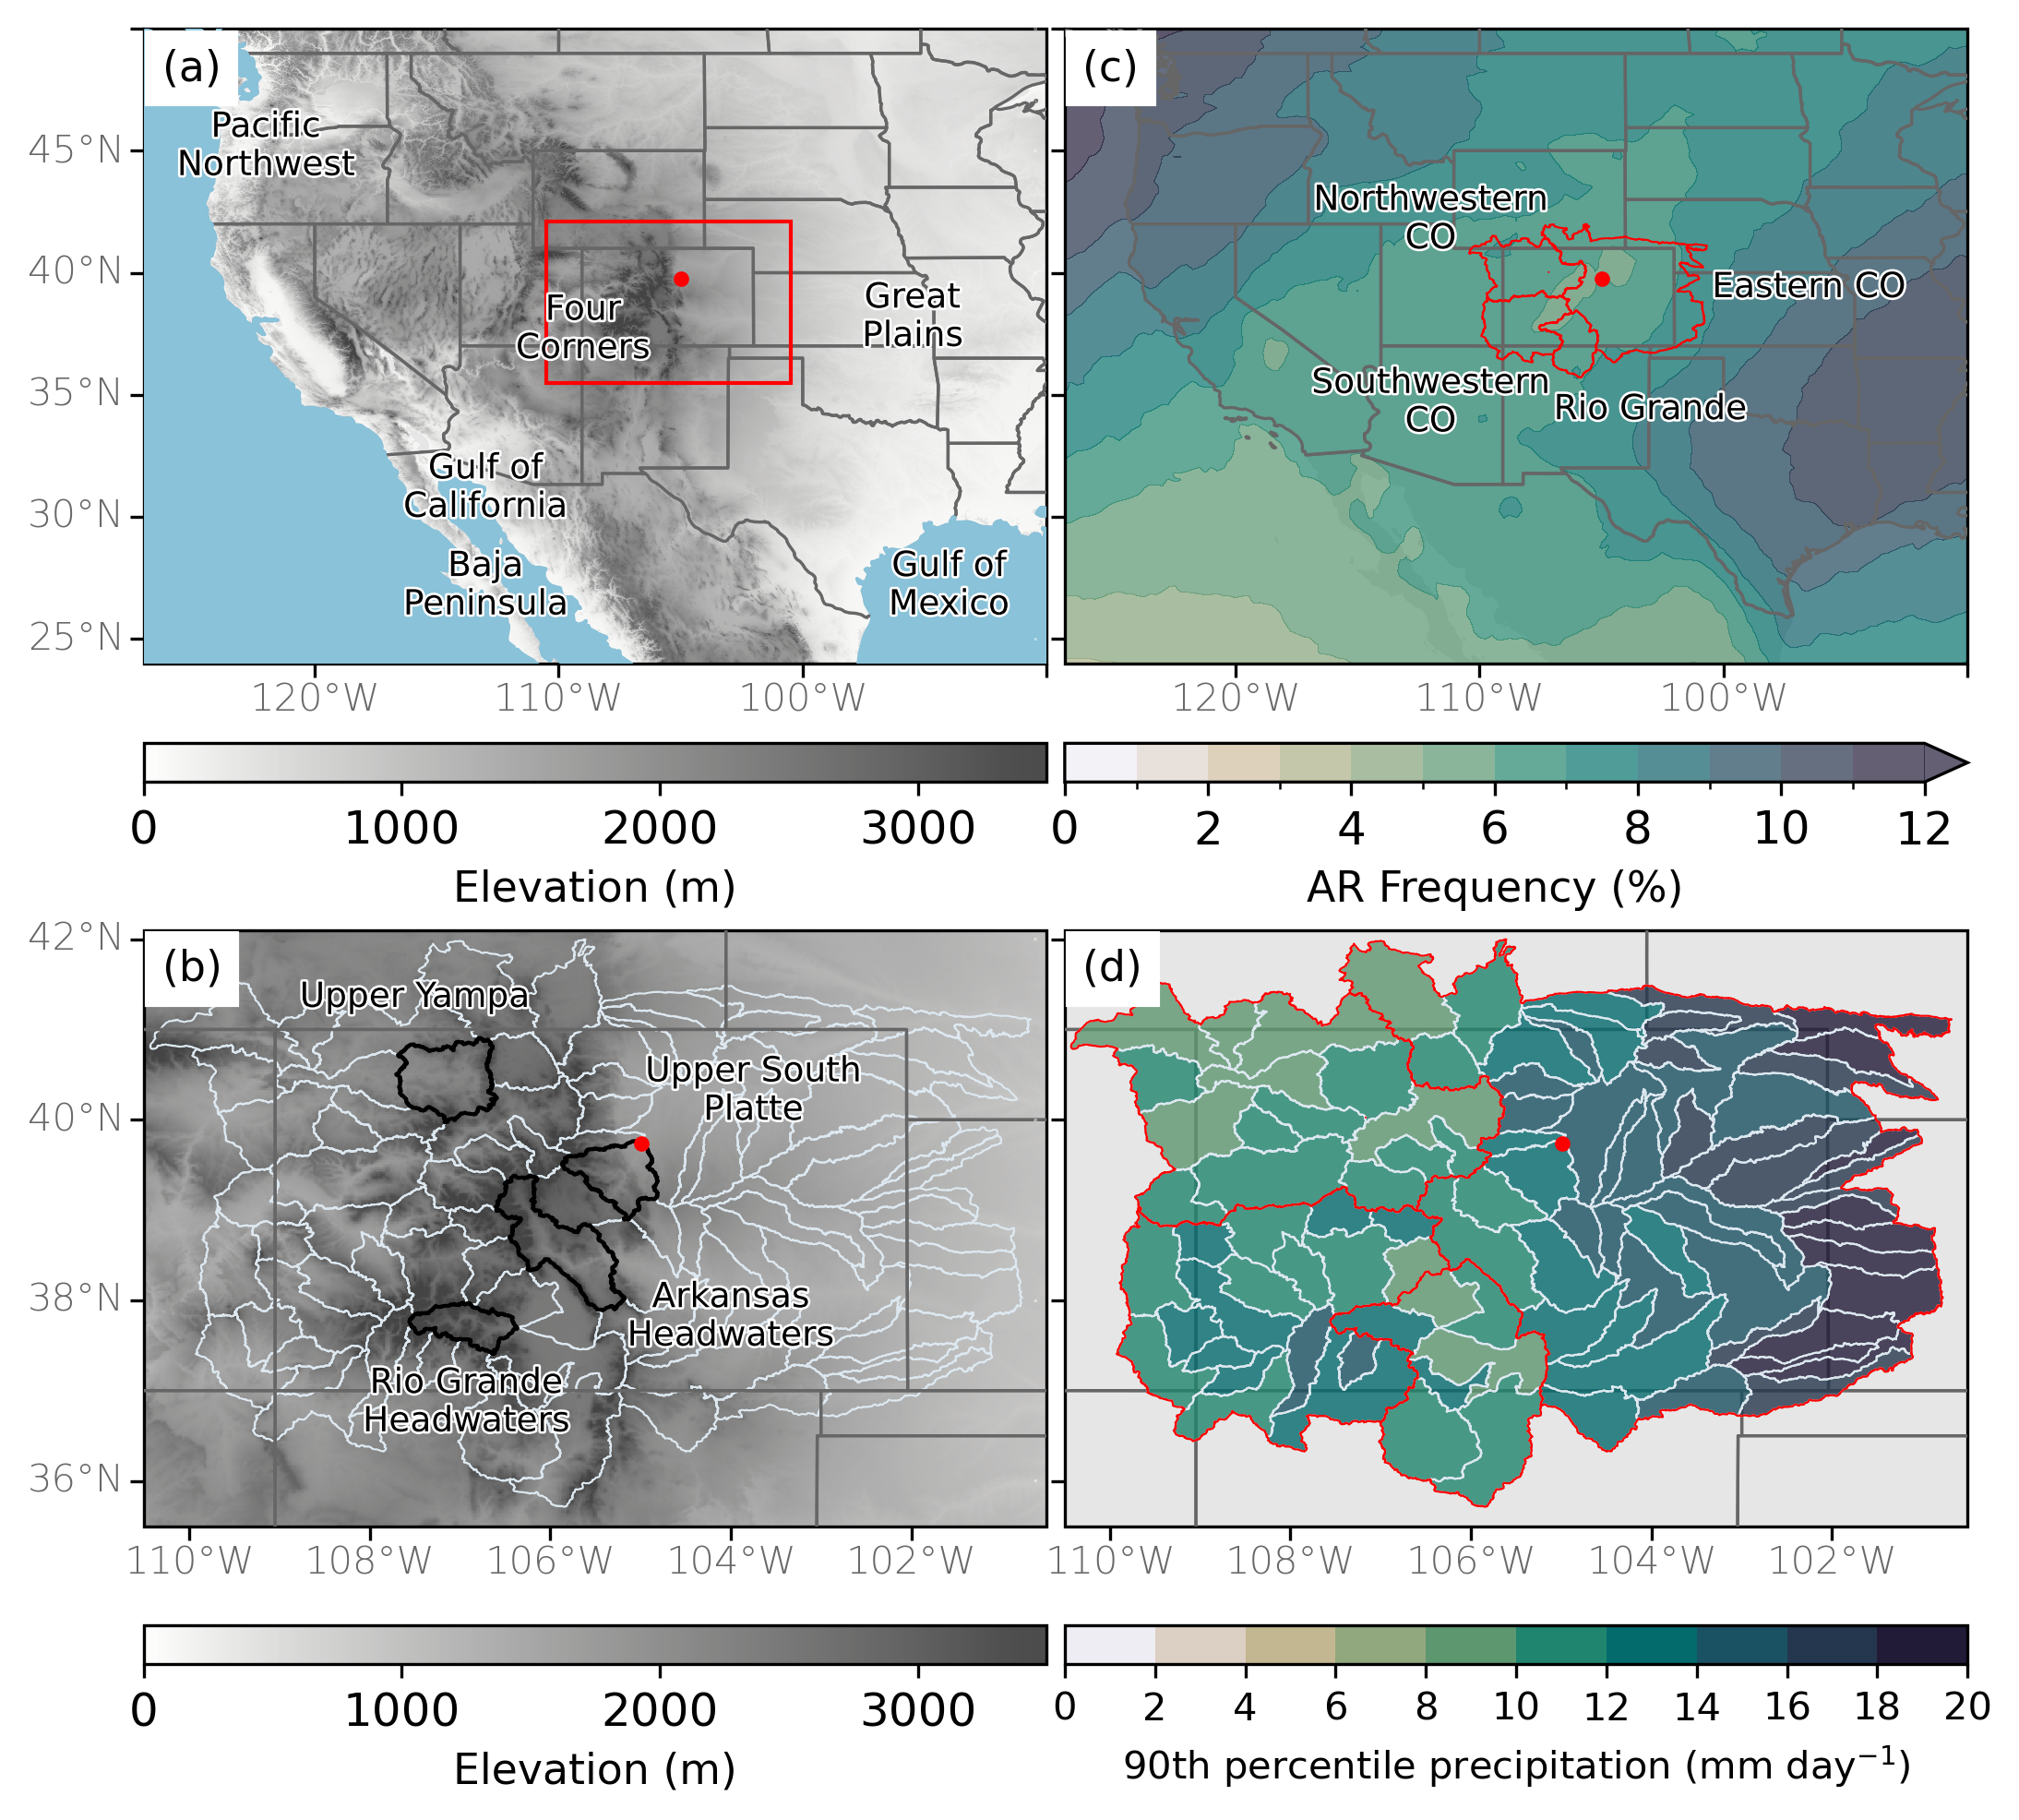
\includegraphics[width=\textwidth, height=\textheight, keepaspectratio]{fig1.png}
\label{fig:ar_overhead}
\caption{Frequency of AR conditions (\%; the fraction of analyses times meeting the criteria)  based on (a) the \citeA{Guan2024AERA5} tARget v4 using ERA5 (1-hr), (b) the AR Scale \cite{MartinRalph2019} using ERA5 (1-hr) and (c) the \citeA{Rutz2014} ARDT using MERRA2 (3-hr). See Section \ref{sec:data} for more information on each ARDT. The black contours are the HU2 Regions, the grey contours are the HU8 subbasins that fall within Colorado, and the red dot indicates the location of Denver.}
\end{figure}

\section{Methods}
\label{sec:methods}
\subsection{Backwards Trajectory Analysis}

To run the backwards trajectories, we use the simple lagrangian analysis employed in \citeA{Rutz2015} where the zonal, meridional, and vertical wind components from ERA5 data are trilinearly interpolated to determine the atmospheric data at each trajectory location for 72 hours at 1-h resolution. The ~27-km horizontal resolution and 1-hr temporal resolution in ERA5 provides a reasonable estimate for the interpolated atmospheric data at each subsequent trajectory location.

We completed sensitivity tests on the grid points, height, and time of initialization conditions for four individual subbasins within each of the basins for four separate, top-decile precipitation days. Figure \ref{fig:sensitivity_tests} shows the results of the varying initialization sensitivity tests for the 17--19 March 2003 storm that produced historical snowfall and significant impacts across Colorado \cite{Wesley2013Extreme2003}. \textbf{Grid Points:} The sensitivity test trajectories were initiated from the latitude and longitude of the centroid of the subbasin, plus at four points (N, S, E, W) that were 0.25\textdegree{} from the centroid (e.g. if the centroid of the subbasin was 107\textdegree W, 38\textdegree N, the additional initialization points were 107\textdegree W, 38.25\textdegree N, 107\textdegree W, 37.75\textdegree N, 106.75\textdegree W, 38\textdegree N, and 107.25\textdegree W, 38\textdegree N). There were few differences in the trajectories initialized from the different grid points; there were a few exceptions in the trajectories initialized from 600 hPa in the Arkansas Headwaters (southeastern CO) (Fig. \ref{fig:sensitivity_tests}e, g, and h) where some of the trajectories were sourced from more northerly flow while others followed a more southerly anticyclonic rotation. Likely these differences arose from differences in surface pressure from the different points, therefore, we chose to run all the trajectories from the centroid of each subbasin.

\textbf{Height:} In the vertical, we examined trajectories initiated on pressure levels from 500 hPa to 800 hPa at 100-hPa increments (e.g., 500, 600, 700, 800) (Fig. S1). The different initialization heights resulted in very different trajectory paths, as the parcel followed the synoptic patterns typical for that height. For example, the trajectories initialized from 500 hPa (Fig. \ref{fig:sensitivity_tests}a--d) exhibit more westerly flow, aligning with typical midlatitude 500 hPa wind patterns. On the other hand, below 700 hPa, 95\% of the trajectories come from the north, likely the barrier jet-like feature identified in \citeA{Wesley2013Extreme2003}. Due to the complex topography of Colorado and the varying results from the different initialization heights, we chose to initialize each trajectory at the single pressure level between 50 and 100 hPa above (at a lower pressure than) the surface. For example, at the grid point closest to the centroid of the Upper Yampa subbasin, the surface pressure was 827 hPa, so the trajectory for that subbasin was initialized from 750 hPa. Meanwhile, at the grid point closest to the centroid of the South Platte subbasin, the surface pressure was 967, so the trajectory for that subbasin was initialized from 850 hPa. This methodology, similarly employed by \citeA{Alexander2015}, initializes trajectories high enough so that the majority of the trajectories remained above the surface over North America, but was low enough to be located within the region of strong water vapor transport (i.e., between 1000 and 300 hPa). 

\textbf{Time:} Since the PRISM daily precipitation data is centered on 00 UTC of each day, the sensitivity test trajectories were initialized at 12 and 18 UTC of the previous day, plus 00, and 06 UTC of the day when precipitation exceeded the 90th percentile. There were few differences in trajectories initialized at different times in the 24-hour period of precipitation accumulation; therefore, we chose to initialize all of our trajectories from 00 UTC to center them in the middle of the 24-hour precipitation accumulation period. 

\begin{figure}
\noindent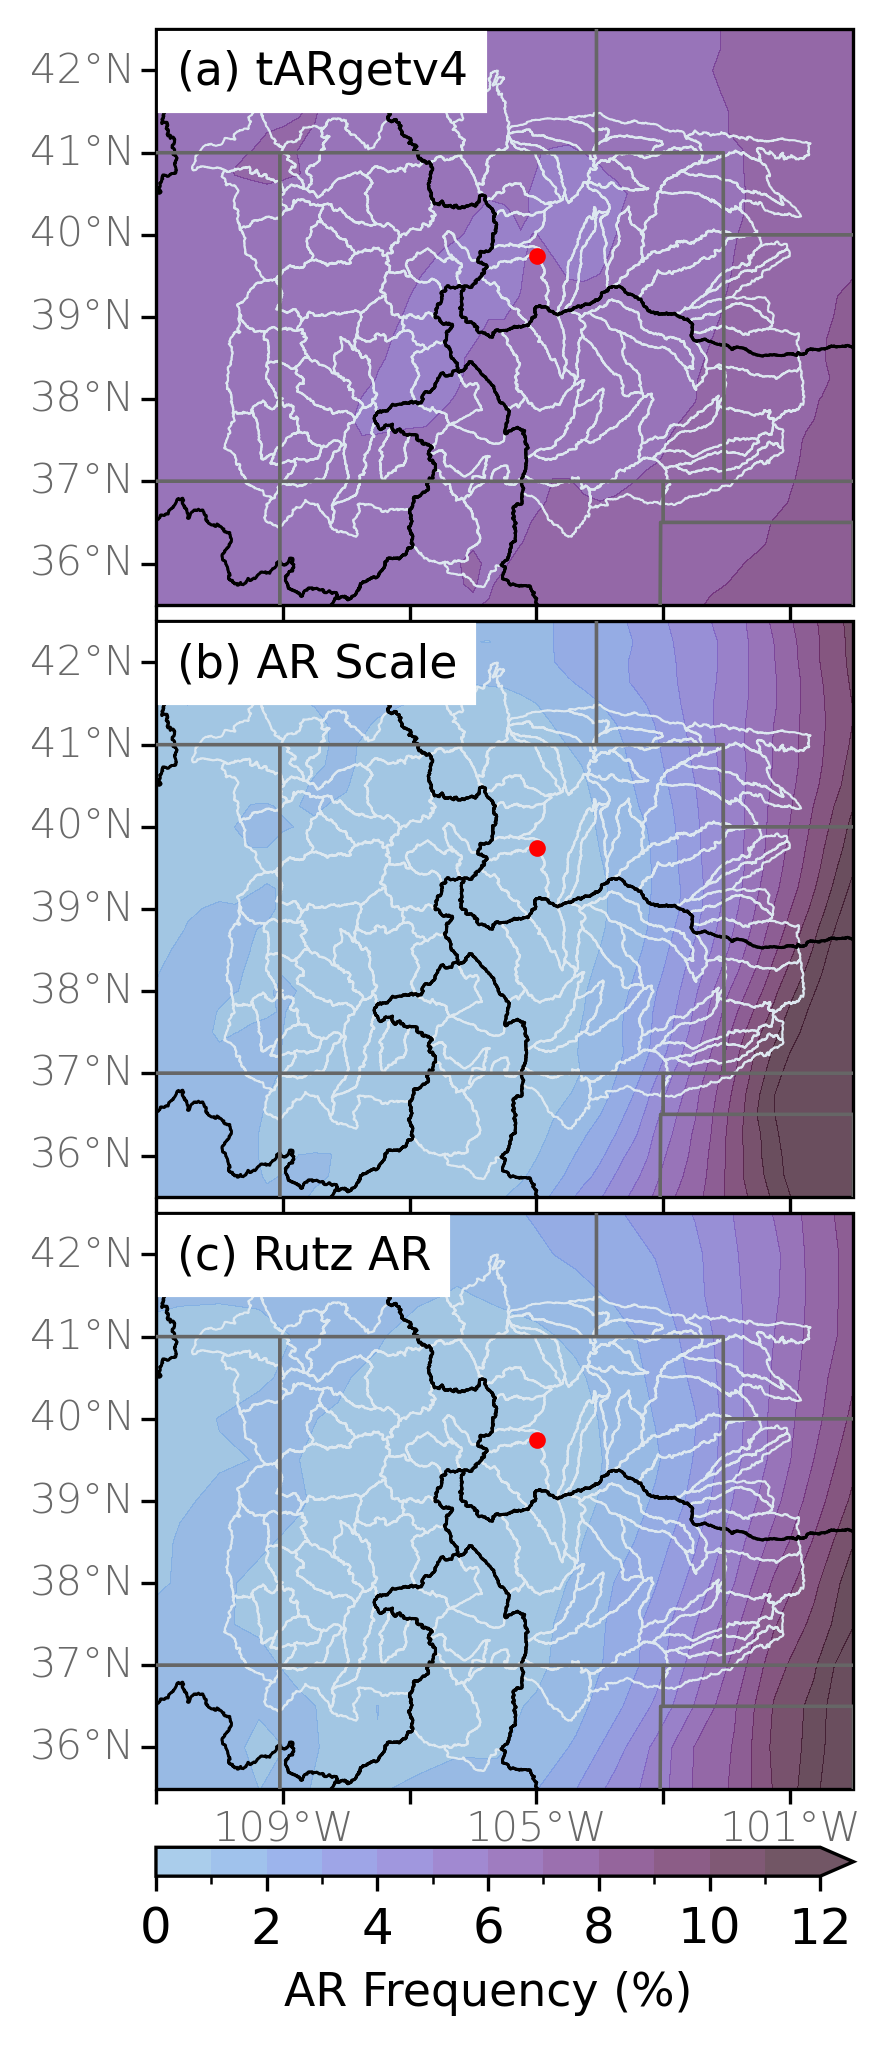
\includegraphics[width=\textwidth]{fig2.png}
\label{fig:sensitivity_tests}
\caption{Examples of backwards trajectories that were initialized from the grid cell closest to the centroid of the Upper Yampa (yellow lines), Upper Dolores (green lines), Upper South Platte (light blue lines) and Arkansas Headwaters (dark blue lines) subbasins, as well as the four grid cells 0.25° north, south, east, and west of the centroids starting at (a-d) 500 hPa, (e-h) 600 hPa, (i-l) 700 hPa, (m-p) 800 hPa. The start time for initialization is indicated by the column where (a, e, i, m) started on 18 March 2003 12Z, (b, f, j, n) 18 March 2003 18Z, (c, g, k, o) 19 March 2003 00Z, and (d, h, l, p) 19 March 2003 06Z. }
\end{figure}

\subsection{AR Conditions at the Coast}
\label{sec:methods:ar_conditions}
To determine whether any given top-decile precipitation day was associated with an AR we evaluated the AR conditions when the trajectory crossed the coast across North America. We tested multiple ARDTs including the AR Scale using ERA5 data \cite{MartinRalph2019}, the \citeA{Rutz2014} ARDT, and the \cite{Guan2024AERA5} tARget v4 ARDT. Overall, there was little variation in the final results and Fig. \ref{fig:choropleth} shows the differences in the ARDTs for the contribution of ARs to top-decile precipitation. Fig. \ref{fig:choropleth} shows the differences in the ARDTs for the contribution of ARs to top-decile precipitation. The \citeA{Rutz2014} ARDT had the least number of ARs at the coast considered to be associated with precipitation in subbasins in western Colorado, likely due the ARDT being based on an absolute IVT threshold, as well as geometry requirements. The \cite{Guan2024AERA5} tARget v4 ARDT had the next highest number of ARs at the coast associated with precipitation in subbasins in western Colorado, likely due to the ARDT being based on a relative IVT threshold, rather than an absolute. On the other hand, subbasins in southeastern Colorado had a higher number of ARs at the coast associated with precipitation from the \citeA{Rutz2014} ARDT compared to the \cite{Guan2024AERA5} tARget v4 ARDT, as a minimum absolute threshold of IVT $>$ 250 kg m\textsuperscript{-1} s\textsuperscript{-1} occurs more frequently over the Gulf of Mexico due to the higher climatological water vapor content. The majority of the trajectories associated with the subbasins in southeastern Colorado were tracked back to the Gulf of Mexico (see Section \ref{sec:results:moisture_pathways} for more discussion). Overall in Colorado, the AR Scale using ERA5 data \cite{MartinRalph2019} had the highest number of ARs at the coast associated with precipitation in Colorado subbasins, likely due to the methodology not having geometry requirements for detecting ARs. For the remainder of the paper, we share the results using the AR Scale using ERA5 data \cite{MartinRalph2019}.

We also tested multiple spatio-temporal criteria for determining whether a trajectory was associated with an AR at the coast. For example, we utilized “strict” requirements for associating a trajectory at the coast with an AR. The strict method said if a trajectory crossed the coast, the AR had to be present at the hour the trajectory crossed the coast as well as at the same grid cell. With the strict methodology, we saw only about xx ARs associated with the Upper Yampa subbasin per year. On the other hand, we used “flexible” criteria to determine whether any given trajectory was associated with an AR. The flexible criteria said that if there was an AR within any grid cell within 1 degree (+- 0.5 degree from the grid where the trajectory crossed the coast) and within 24 hours (+- 12 hours from when the trajectory crossed the coast). The flexible requirements saw about 20 ARs associated with the Upper Yampa subbasin per year. In the end, we chose to utilize the flexible requirements for this analysis. This is because the trajectories themselves are fairly ephemeral and are tracking one specific air parcel in space in time that we assume is associated with the precipitation in that subbasin. Based on our sensitivity tests on initialization conditions, you can see that even with minor changes in initialization conditions can result in a different end point for the trajectory. Therefore, using the flexible requirements for determining whether that top-decile precipitation day is associated with a coastal landfalling AR is better for capturing the possibility that even though that exact air parcel does not have an AR directly overhead at the coast, it is likely that the moisture from the AR was able to penetrate inland and reach Colorado and result in precipitation.

\begin{figure}
\noindent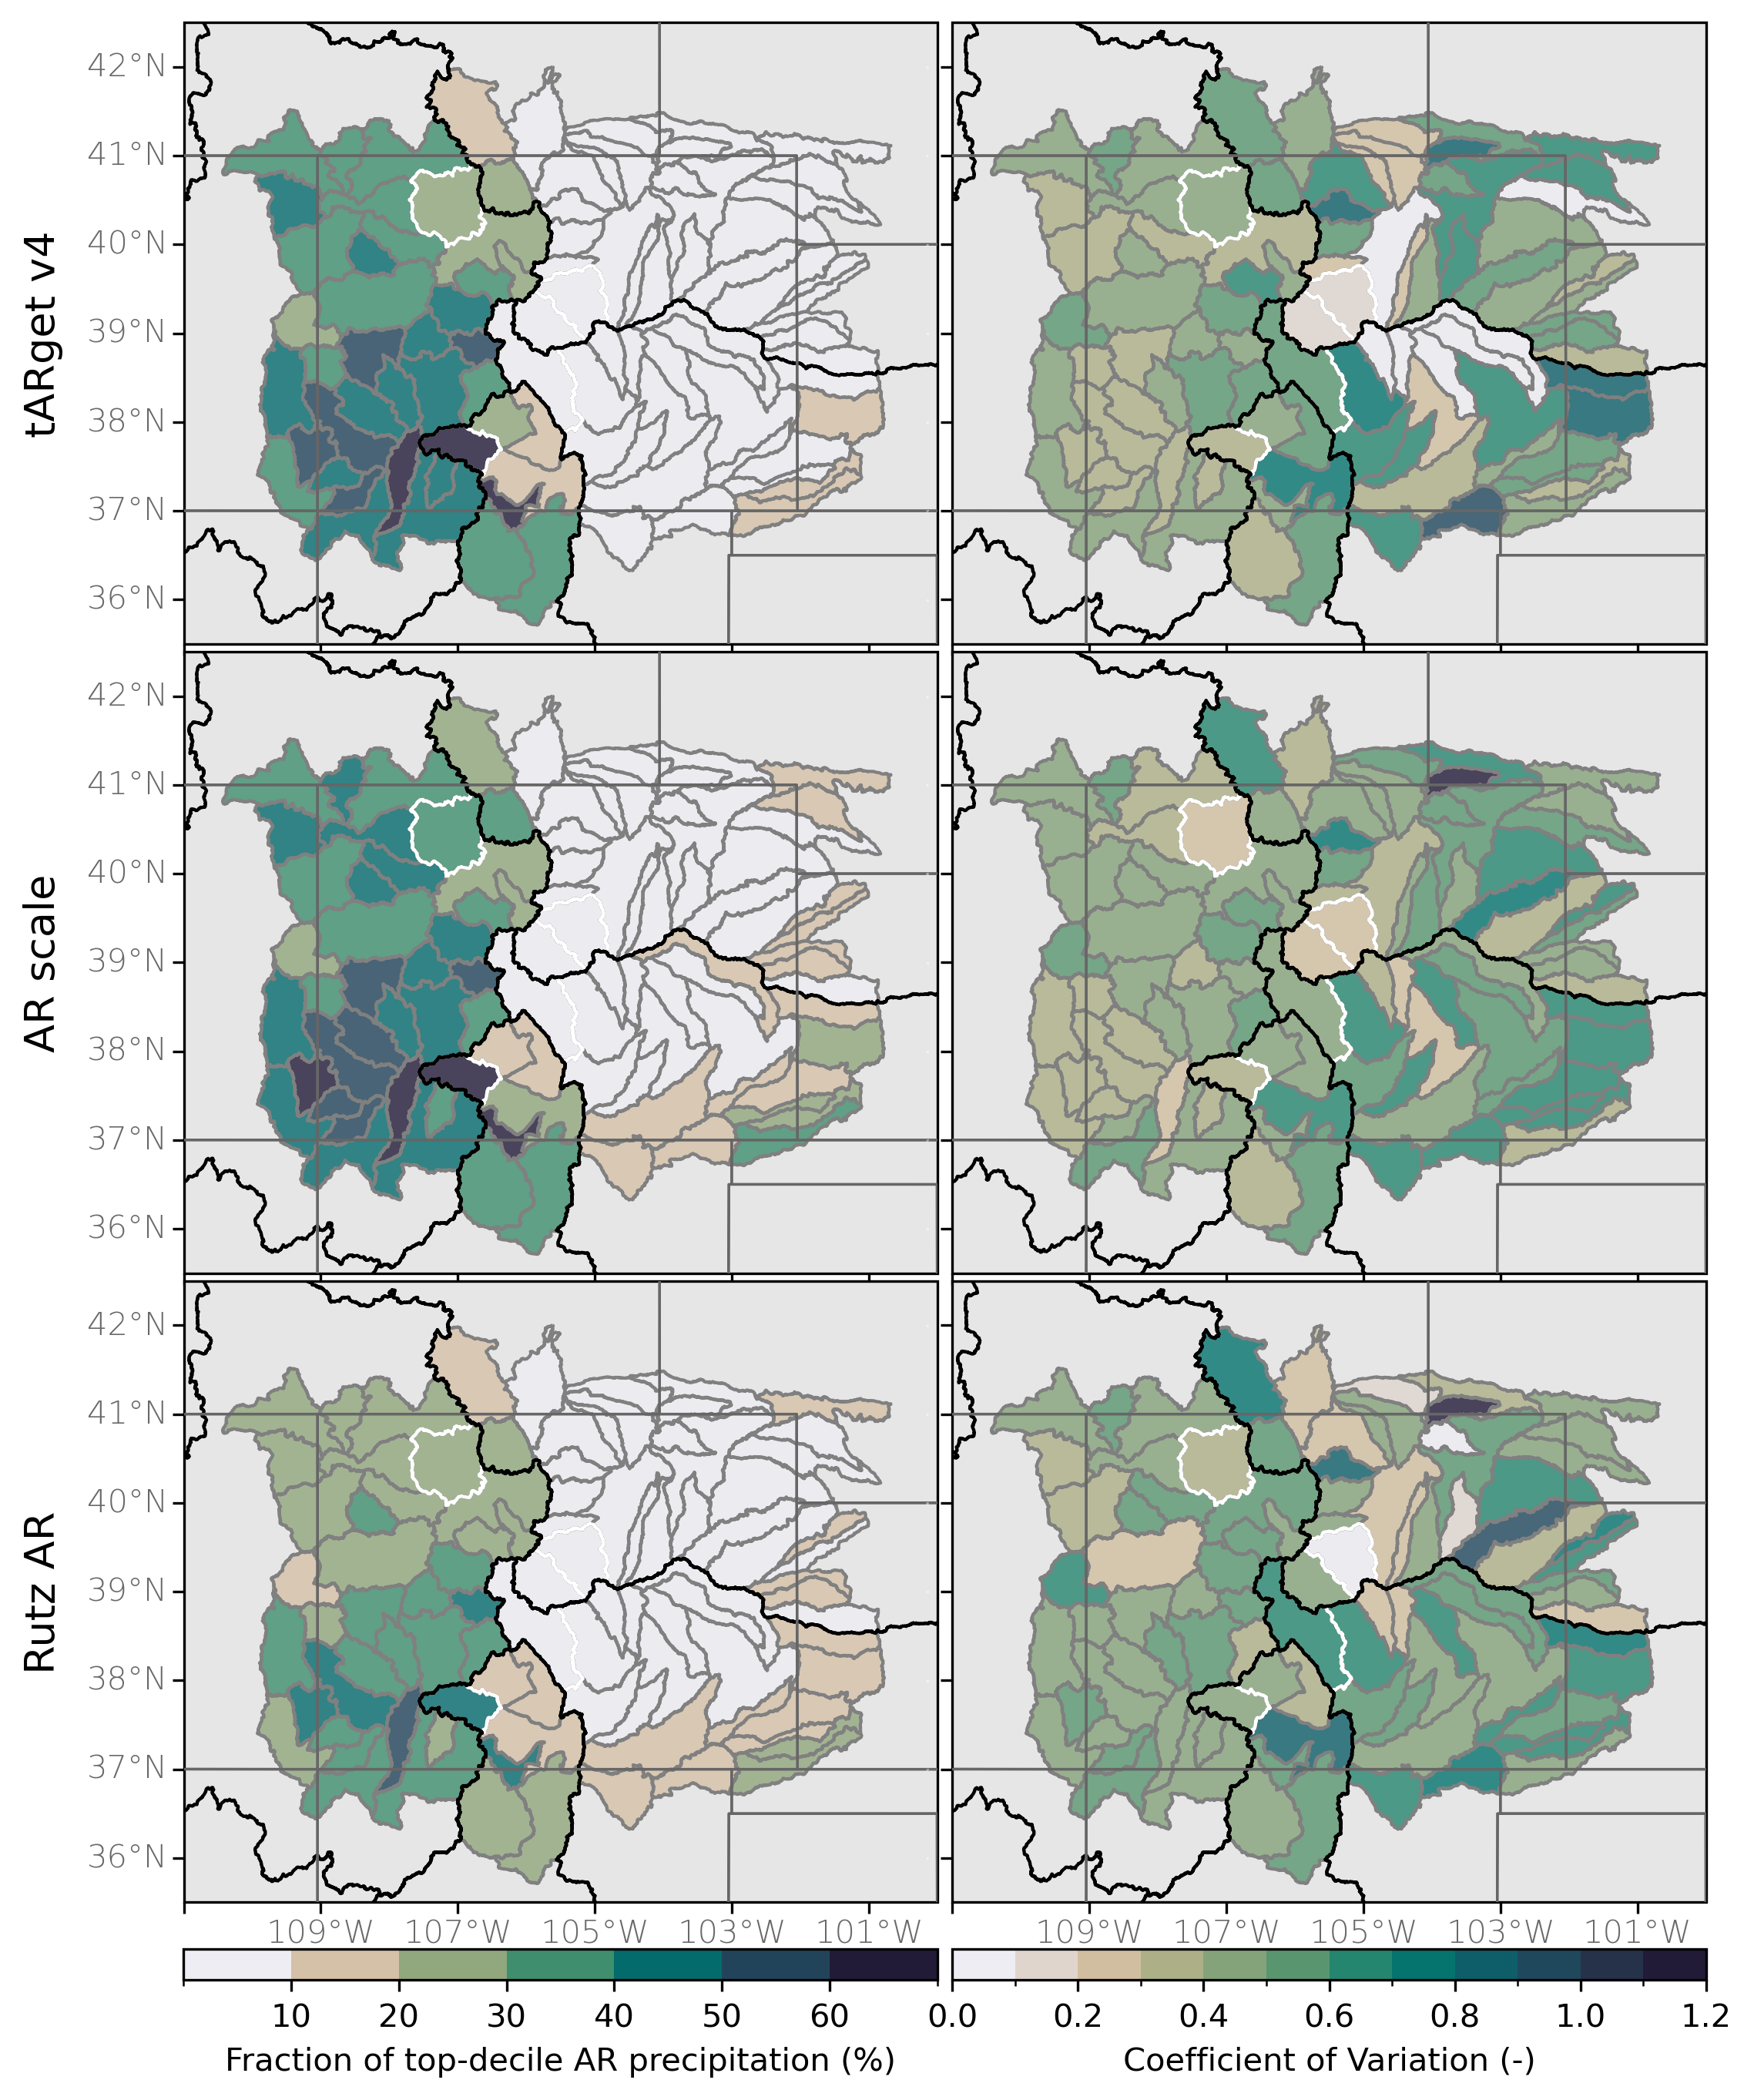
\includegraphics[width=\textwidth]{fig3.png}
\label{fig:choropleth}
\caption{(a–c) The fraction of top-decile precipitation associated with coastal landfalling ARs (shaded; \% of total top-decile precipitation between 2000 and 2023) for each subbasin (contour, grey) in Colorado based on (a) tARgetv4 (Guan and Waliser, 2015), (b) ERA5 AR Scale (Ralph et al., 2019), and (c) Rutz et al., (2014) ARDT. The white highlighted subbasins are the Upper Yampa (northwest), Upper Dolores (southwest), Upper South Platte (northeast), and Arkansas Headwaters (southeast). The black contours indicate the HU2 Regions that each subbasin falls within. (d–f) The standard deviation of the fraction of top-decile precipitation within each water year associated with coastal landfalling ARs (shaded; \%) for each subbasin (contour, grey) in Colorado based on (d)  tARgetv4 (Guan and Waliser, 2015), (e) ERA5 AR Scale (Ralph et al., 2019), and (f) Rutz et al., (2014) ARDT. }
\end{figure}

% \section{Materials and Methods}
% Here is text on Materials and Methods.
%
% \subsection{A descriptive heading about methods}
% More about Methods.
%
%
% \section{Results} (Or section title might be a descriptive heading about the
% results)
\section{Results}

\subsection{Contribution of AR moisture to Top-Decile Precipitation events across Colorado}
\label{sec:results:contribution}
% Main Idea: This section will describe the contribution (average and interannual variation) of AR moisture to top-decile precipitation events across Colorado
% Introduce: Using the above-defined methodology for backwards trajectory analysis and determining if each trajectory was associated with an AR when it crossed the coast or not, Figure 3 shows the fraction of top-decile precipitation associated with landfalling AR moisture. 
% Key Point: Describe the results of the various ARDTs
% Explain Key Point: This point needs to be made to show that even with varying ARDTs, the results are consistent. Then describe the patterns of fraction of contribution with an emphasis on NW, SW, NE, SE Colorado
% Connect: This map directly represents the total top-decile precipitation contribution by moisture associated with ARs between 2000 and 2023 for each subbasin. 
% Next Key Point: Compare the results to those found in Rutz et al. 2015
% Explain Key Point: The results we have show a higher fraction of contribution - this aligns with anecdotal evidence from NWS and shows that this is a useful methodology for identifying AR moisture penetrating inland in locations that do not see as much AR activity. Additionally, add a sentence or two about the SNOTEL station result in the San Juans in Rutz et al. 2015 and how that aligns very well with what our results show.
% Connect: This shows that our methodology is an improvement, but also still aligns well with previous research - this methodology could be used elsewhere and is needed in CO.
% Next Key Point: Describe the number of trajectories associated with a landfalling atmospheric river (Figure 4)
% Explain Key Point: This result shows the paths and AR scale value associated with the trajectories that did cross the coast broken down by season - this gives us a general number per year of top-decile precipitation days associated with atmospheric river moisture and starts to give us an idea of the paths moisture takes for the different basins across Colorado
% Connect: This shows when AR associated moisture is more frequent for each basin in Colorado as well as starts to show the paths that they take (i.e., winter westerly trajectories more common for western CO while summer southeasterly trajectories are more common for eastern CO)

For all top-decile precipitation days in each of the 92 subbasins in Colorado, we applied the backwards trajectory analysis as outlined in Section \ref{sec:methods} and then determined AR conditions at the coast using three different ARDTs: tARgetv4, Rutz ARDT, and ERA5 AR Scale \cite{MartinRalph2019, Rutz2014, Guan2024AERA5}. Figure \ref{fig:choropleth} shows the fraction of top-decile precipitation associated with coastal landfalling ARs for each of the different ARDTs and their coefficient of variation for contributions from water year to water year. 

%% sentences about the higher fraction located in western CO
In western Colorado, in the Colorado and Rio Grande Regions, moisture from coastal landfalling ARs is associated with 10--70\% top-decile precipitation, with the highest fraction of top-decile precipitation associated with ARs occurring in subbasins in southwestern Colorado (Fig. \ref{fig:choropleth}a--c). The subbasins with the highest contribution are Animas subbasin with 69.4\%, Conejos subbasin with 60.3\%, and Upper Dolores subbasin with 59.5\%. In the Rio Grande Headwaters, the contribution is 65.4\%, a much higher fraction than the 0--30\% of contribution that \citeA[Fig. 11b]{Rutz2014} found in southwestern Colorado. The differences between these results is likely because \citeA{Rutz2014} calculates the fraction of top-decile precipitation associated with ARs directly overhead using the Rutz ARDT, which has geometry requirements and an absolute IVT threshold of 250 kg m\textsuperscript{-1} s\textsuperscript{-1}. IVT in western Colorado averages around 100 kg m\textsuperscript{-1} s\textsuperscript{-1} and peaks around 500 kg m\textsuperscript{-1} s\textsuperscript{-1}, therefore, it would be rare for IVT to exceed 250 kg m\textsuperscript{-1} s\textsuperscript{-1}, let alone an AR maintain its shape long enough across western Colorado to meet the geometry requirements. In \citeA[Fig. 3]{Rutz2015}, they run forward trajectory analysis from the U.S. West Coast on AR landfall days and found that less than 130 trajectories classified as coastal-decaying ARs were able to reach Colorado, while fewer than 50 interior-penetrating AR trajectories reached Colorado.

In the Rio Grande Headwaters, there was very little variability in the fraction of top-decile AR precipitation between the tARgetv4 and AR Scale ARDTs where the fraction was about 63\% and 65\%, respectively, while the fraction for the Rutz ARDT was much lower at 47\% (Fig. \ref{fig:choropleth}a--c). For more discussion on the differences in the ARDTs, see Section \ref{sec:data} and \ref{sec:methods:ar_conditions}. The water year coefficient of variability ranged from 0.3 (based on AR Scale ARDT, Fig. \ref{fig:choropleth}e) to 0.4 (based on Rutz ARDT, Fig. \ref{fig:choropleth}f) in the Rio Grande subbasin.

In northwestern Colorado, AR moisture is associated with 20--50\% of the total top-decile precipitation, with about 35\% in the Upper Yampa subbasin (white outline in northwest CO). There is little variation between the different ARDTs and the fraction of AR-associated top-decile precipitation. In the Upper Yampa subbasin, the tARgetv4 and Rutz ARDTs found the lower fraction of top-decile AR precipitation at 25\% and 27\%, respectively (Fig. \ref{fig:choropleth}a, c), while the AR Scale ARDT fraction was higher at 35\% (Fig. \ref{fig:choropleth}b). For year to year variability, the coefficient of variability ranged from 0.3 (based on AR Scale ARDT, Fig. \ref{fig:choropleth}e) to 0.4 (based on tARgetv4 ARDT, Fig. \ref{fig:choropleth}d) in the Upper Yampa subbasin. \citeA{Lute2014RoleStates} suggest that the similar variability in the fraction of top-decile precipitation from water year to water year in the Upper Yampa and Rio Grande subbasins is likely due to the high elevation of these regions and most of the precipitation accumulation occuring during winter months. 

Contributions are lower in eastern Colorado, ranging from 0--40\%. In northeastern Colorado, in the Upper South Platte subbasin, contributions from ARs to top-decile precipitation are less than 5\%, but there is some variability between ARDTs (Fig. \ref{fig:choropleth}a--c). The Rutz ARDT identified the lowest fraction at 0.6\% (Fig. \ref{fig:choropleth}c), tARget at 2.5\% (Fig. \ref{fig:choropleth}a), and the AR Scale at 4\% (Fig. \ref{fig:choropleth}b). However, there is very little water year variability in the Upper South Platte, with coefficients from the different ARDTs ranging from 0--0.2 (Fig. \ref{fig:choropleth}d--f). This is likely because there are very few trajectories that are associated with ARs in this region in the first place. 

Southeastern Colorado sees a higher contribution over a larger area than northeastern Colorado, with 10--40\% of top-decile precipitation associated with coastal AR moisture (Fig. \ref{fig:choropleth}a--c). There was very little variability between ARDTs in the fraction of top-decile AR precipitation in the Arkansas Headwaters subbasin, where the tARgetv4 and Rutz ARDTs found a slightly lower fraction of top-decile AR precipitation at 8.5\% and 8\%, respectively (Fig. \ref{fig:choropleth}a, c), compared to the AR Scale ARDT fraction at 9.5\% (Fig. \ref{fig:choropleth}b). Most of the variability between the ARDTs occurs in the most southeasterly subbasins in Colorado, with tARgetv4 identifying a lower contribution than Rutz ARDT and the AR Scale (Fig. \ref{fig:choropleth}d--f).

This is likely because the main difference between the ARDTs is that tARgetv4 uses a relative, percentile-based threshold for determining the minimum IVT value to be considered part of an AR and Rutz ARDT and ERA5 use an absolute threshold of 250 kg m\textsuperscript{-1} s\textsuperscript{-1}. Since a large fraction of the trajectories in southeastern Colorado sourced moisture from the Gulf of Mexico (see Section \ref{sec:results:moisture_pathways} for more discussion on the moisture pathways), a relative threshold like the one used in tARgetv4 is likely to detect fewer ARs, while an absolute threshold will detect more ARs because IVT values are climatologically a lot higher. In northeastern Colorado, only two subbasins located in the far northeastern region of the state see contributions higher than 10\%. 

Water year variability coefficients are some of the highest in the Arkansas Headwaters subbasin, ranging from 0.5 (tARgetv4 and AR Scale, Fig. \ref{fig:choropleth}d, e) to 0.6 (Rutz ARDT, Fig. \ref{fig:choropleth}f). This is likely because extreme precipitation in the Arkansas River basin falls primarily during convective storms in warm season months, and has high spatial heterogeneity due to complex terrain \cite{Javier2007ClimatologyBasin}.

Figure \ref{fig:time_series} shows the top-decile precipitation within each water year (WY) for the Upper Yampa, Rio Grande Headwaters, Upper South Platte, and the Arkansas Headwaters subbasins and compares them to the contribution associated with coastal ARs. Notably, the fraction of top-decile precipitation is higher in the Upper Yampa (10--54\%) and Rio Grande Headwaters (31--100\%) subbasins compared to the Upper South Platte (14--20\%) and Arkansas Headwaters (11-25\%) subbasins. Additionally, there are more years in the eastern subbasins where there is a 0\% contribution from coastal ARs to top-decile precipitation, whereas in the Upper Yampa there are 3 years with a 0\% contribution and no years in the Rio Grande Headwaters subbasin. The average amount of top-decile precipitation associated with coastal ARs ranges from just below ~25 mm per year in the Upper Yampa, Upper South Platte, and Arkansas Headwaters subbasin to ~90 mm per year in the Rio Grande Headwaters subbasin. From year to year, there is high variability in top-decile precipitation across all the subbasins. For example, in the Rio Grande Headwaters, the years 2002 and 2018 saw only ~30 mm of top-decile precipitation, while 2001 and 2008 saw 195 mm and 267 mm, respectively. 

\begin{figure}
\noindent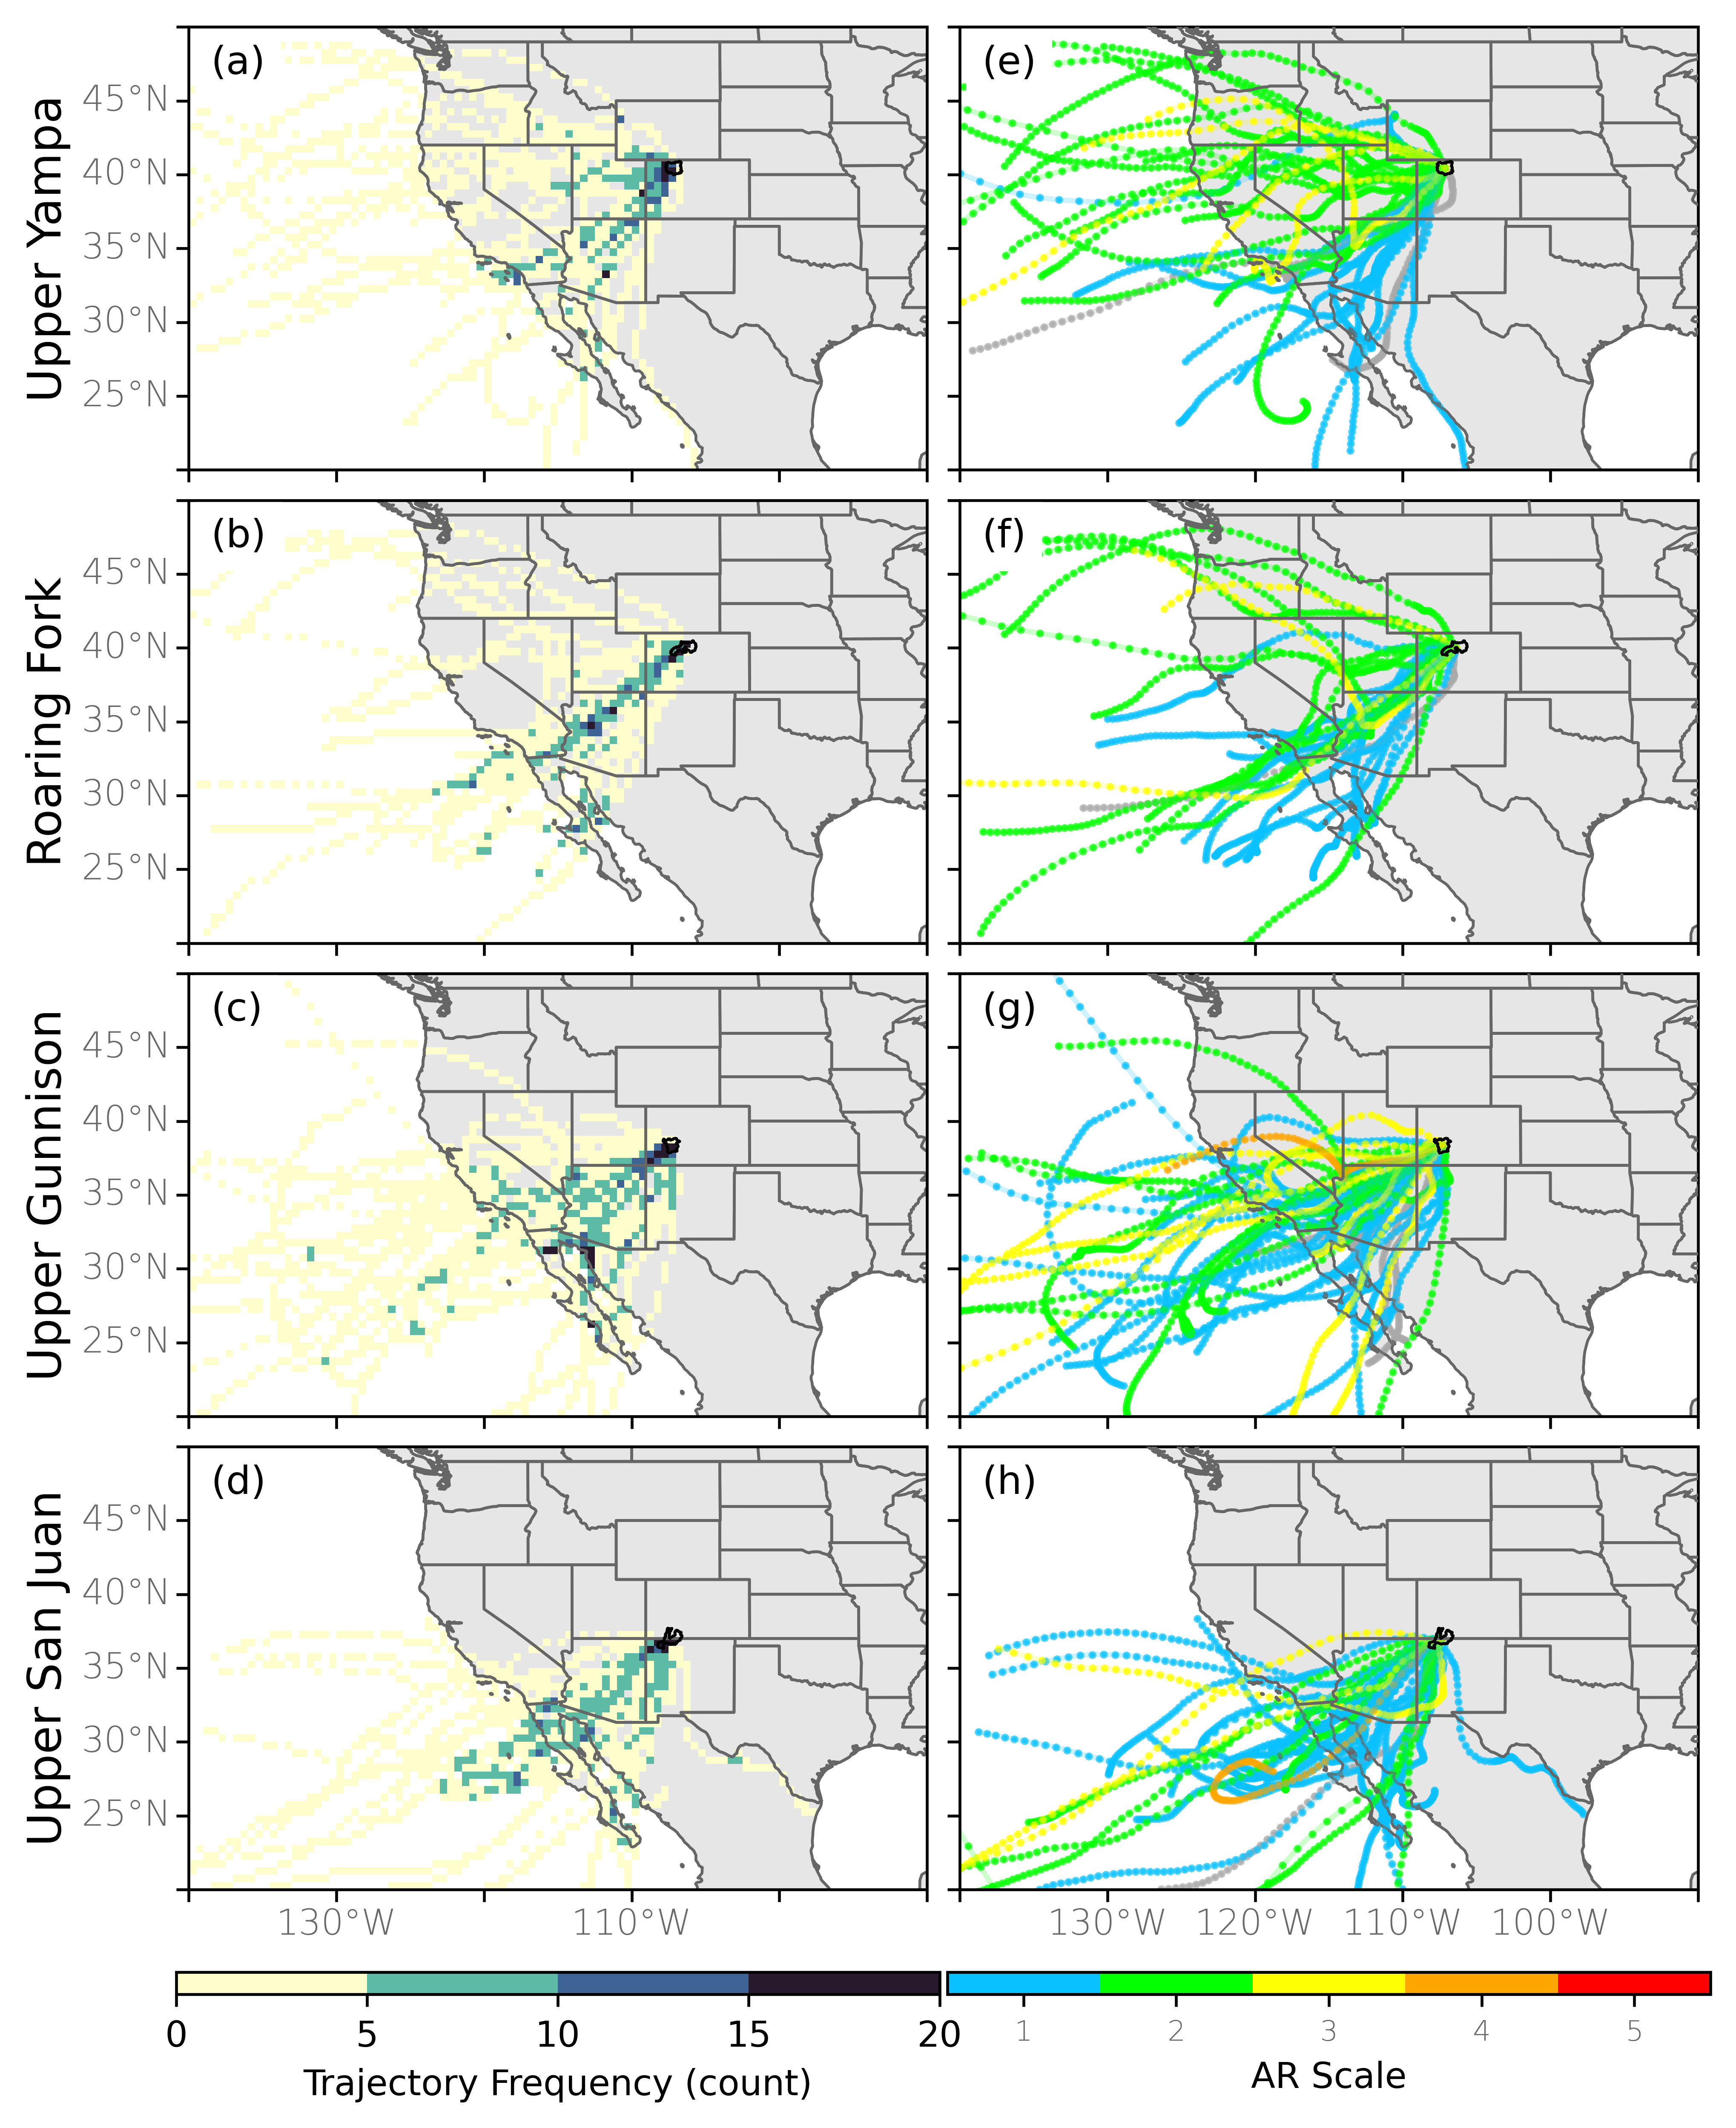
\includegraphics[width=\textwidth]{fig4.png}
\label{fig:time_series}
\caption{(a) Total top-decile precipitation (light red shading; inches per year) within each water year (e.g. WY 2000 indicates from 1 October 1999 to 30 September 2000) for the Upper Yampa subbasin. The dark red shading is the top-decile precipitation in that water year associated with coastal landfalling ARs. The dotted black lines are showing the minimum and maximum contribution to top-decile precipitation. The black solid line is the mean contribution to top-decile precipitation. (b) Same as (a), but for the Upper Dolores subbasin. (c Same as (a) but for the Upper South Platte subbasin. (d) Same as (a) but for the Arkansas Headwaters subbasin. ** note: add percent contribution, min/max, median/mean}
\end{figure}

\subsection{Moisture Pathways for Inland Penetrating ARs}
\label{sec:results:moisture_pathways}
% Main Idea: The main idea for this section is to show the common pathways for moisture to be able to penetrate inland and make it to CO. What are the common paths? What does the vertical structure of the moisture flux look like when it crosses complex topographic areas of interest?
% Introduce: Understanding the moisture paths of the inland penetrating moisture will help us understand the paths more likely to be taken - when forecasts show that ARs are likely to take these paths, we will have a better idea of upcoming precipitation patterns. 
% Key Point: Describe the pathways of moisture using Figure 5 for the different basins and the average IVT as each trajectory passes through (Figure 6).
% Explain Key Point: This will have discussions on the higher frequency of the moisture paths for each basin and what season/time of year is more likely for these paths.
% Connect: We can show that the pathways are very similar to those outlined in Rutz et al., 2015 - however the trajectories from that work did not quite extend to Colorado - this work is confirming the pathways and the relationship to top-decile precipitation.
% Next Key Point: Now that we have the horizontal pathways described, we now will show the vertical pathway composites over a few topographic areas of interest (e.g., where the horizontal pathways are common and there are topographic barriers) (Figure 7)
% Explain Key Point: The vertical pathway composites will show the frequency of the trajectories in the vertical along different topographic barriers of interest. This will give us a better understanding of how the moisture is able to continue penetrating inland - is it along a valley? Is the moisture much higher at a certain point because it has been lifted?
% Connect: This section will give us a better understanding of the vertical structure of the moisture as it penetrates inland.
%

Figures \ref{fig:choropleth} and \ref{fig:time_series} are showing the relative contribution of coastal landfalling ARs to top-decile precipitation in various subbasins in Colorado. Next, we show the common pathways that the trajectories that are associated with coastal landfalling ARs and top-decile Colorado precipitation. To better summarize our findings, we group the subbasins into the regions that they fall in. Colorado has 4 regional basins: Colorado, Rio Grande, South Platte, and Arkansas (see Fig. \ref{fig:ar_overhead} for the extent of each region). We also differentiate between trajectories that occur in the cool-season months (i.e., November 1 through April 30) and warm-season months (i.e., May 1 thorugh October 31). Figure \ref{fig:spaghetti_plot} shows the top-decile precipitation trajectories that are associated with coastal landfalling ARs, with the colors indicating the ERA5 AR scale value when the trajectory crosses the coast. 

By far the Colorado region has the most trajectories associated with ARs at the coast. Of the XX trajectories ran for the xx subbasins, xx were associated with ARs at the coast during the cool-season, and xx during the warm season. In the cool season, AR scale 1 and 2 are the most common with xx trajectories, while there were xx, xx, and xx trajectories associated with AR scale 3, 4, and 5, respectively. The warm season had a similar number of AR Scale 1 and 2 trajecories (xx and xx), but there were only xx trajectories associated with AR scale 3, 4, and 5. Through visual inspection, most of the trajectories from the Colorado region crossed the U.S. West Coast in both the cool-season and warm-season. Less than 10 trajectories in the Colorado region crossed the Gulf of Mexico Coast during the cool-season, and about xx during the warm season. 

The Rio Grande region had the second most trajectories associated with ARs at the coast, with XX trajectories of the XX ran for the xx subbasins during the cool season, and xx during the warm season. REPEAT FOR ALL THE REGIONS

\begin{figure}
\noindent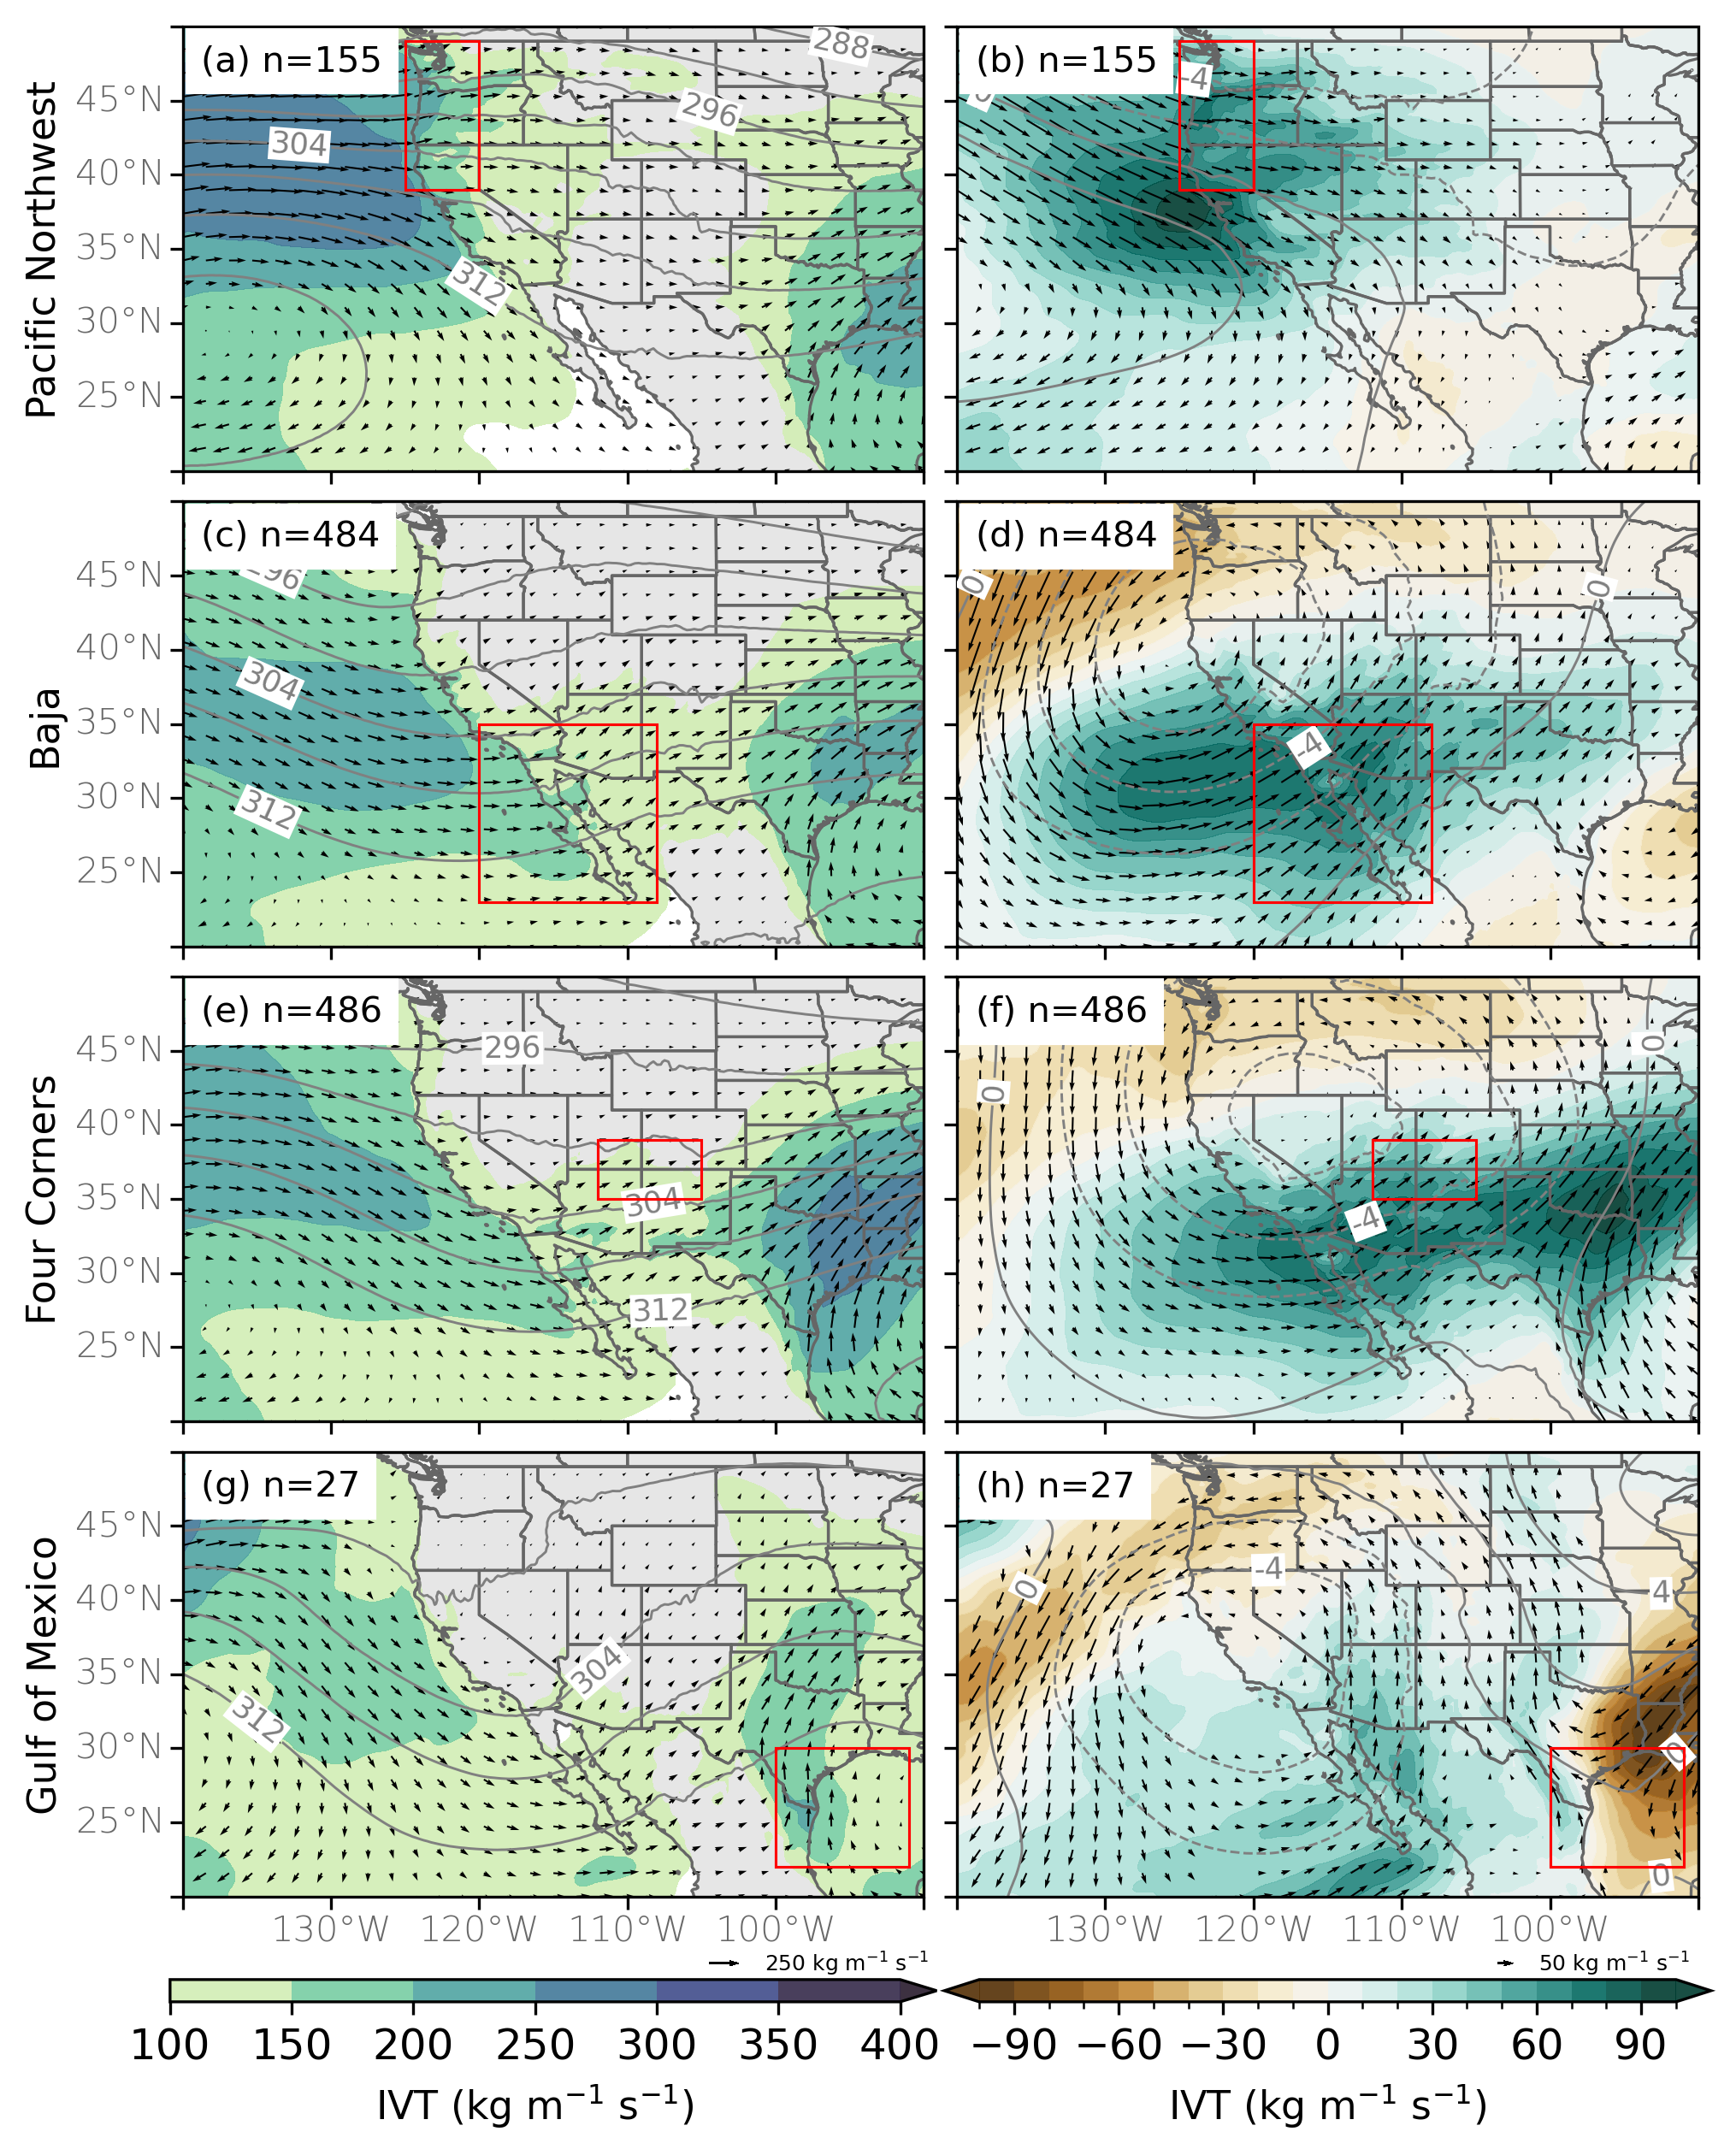
\includegraphics[width=\textwidth]{fig5.png}
\label{fig:spaghetti_plot}
\caption{(a) The backwards trajectories for all Colorado subbasins that fall within the Colorado region (black contour) for the months of November to April from 2000 to 2023 that were associated with an AR defined by the ERA5 AR Scale (Ralph et al., 2019) when the trajectory crossed the coast. (b) Same as (a) but for the Rio Grande region. (c) Same as (a) but for the South Platte region. (d) Same as (a) but for the Arkansas region. (e) Same as (a) but for the months of May to October. (f) Same as (e) but for the Rio Grande region. (g) Same as (e) but for the South Platte region. (h) Same as (e) but for the Arkansas region.}
\end{figure}


To show the preferred pathways of the trajectories that are associated with a coastal landfalling AR, Figure \ref{fig:heatmaps} shows the normalized (using the min-max method) frequency a trajectory point crosses each grid, again broken down by region and warm or cool season, similar to Fig. \ref{fig:spaghetti_plot}. In the Colorado region, the dominant pathway for the trajectories in the cool season is to enter by crossing southern California or the Baja Peninsula, then crossing Arizona and entering Colorado via the southwest corner. There are also quite a few trajectories that appear to enter via the Gulf of Califoria. During the warm months, the preffered pathway is to enter via the Gulf of California, then similar to the path during the cool months, cross Arizona, then enter Colorado through the southwest corner. 

In the Rio Grande region, the preferred pathway during the cool months is similar to that of the Colorado region, albeit with less frequency overall, and very few trajectories crossing the southern California coast. During the warm months, the pathway is again similar to that of the Colorado region, however with a lower frequency. Additionally, there is a higher frequency of trajectories coming in from the Gulf of Mexico coast along the southern border of Texas, crossing New Mexico and entering Colorado in the southcentral region of the state. 

In the South Platte region during the cool months, there is a higher frequency of trajectories entering around southern California and the northern Baja Penisula. Some of the trajectories cross Arizona, but it appears the preferred pathway is to cross the Wahsatch Range in Utah, then northern Colorado before reaching the South Platte region. The complex terrain of the Wahsatch and Park ranges is likely why there are fewer trajectories overall that reach the South Platte region during the cool months, as the water vapor flux likely is reduced dramatically as it is forced to ascend these ranges. The warmer months is when the South Platte region sees a higher frequency of trajectories, with most of the trajectories entering via the Gulf of Mexico coast, crossing Texas, Oklahoma and Nebraska before moving west into the South Platte region. This pathway aligns with some of the historically significant storms that occurred during the spring months along the Front Range, including the March 2003 Blizzard (see Fig. \ref{fig:sensitivity_tests}) and the March 2019 Bomb Cyclone (add Jerry's reference??). 

There are so few trajectories that reach the Arkansas region during the cool months that it is difficult to pin down a preferred pathway. However, during the warm months, the preferred trajectory pathway is very similar to that of the South Platte region during the warm months, again, aligning well with the known synoptic patterns of historically significant spring storms, but also the synoptic patterns associated with summertime short duration convective storms that often get their moisture from the Gulf of Mexico. 


\begin{figure}
\noindent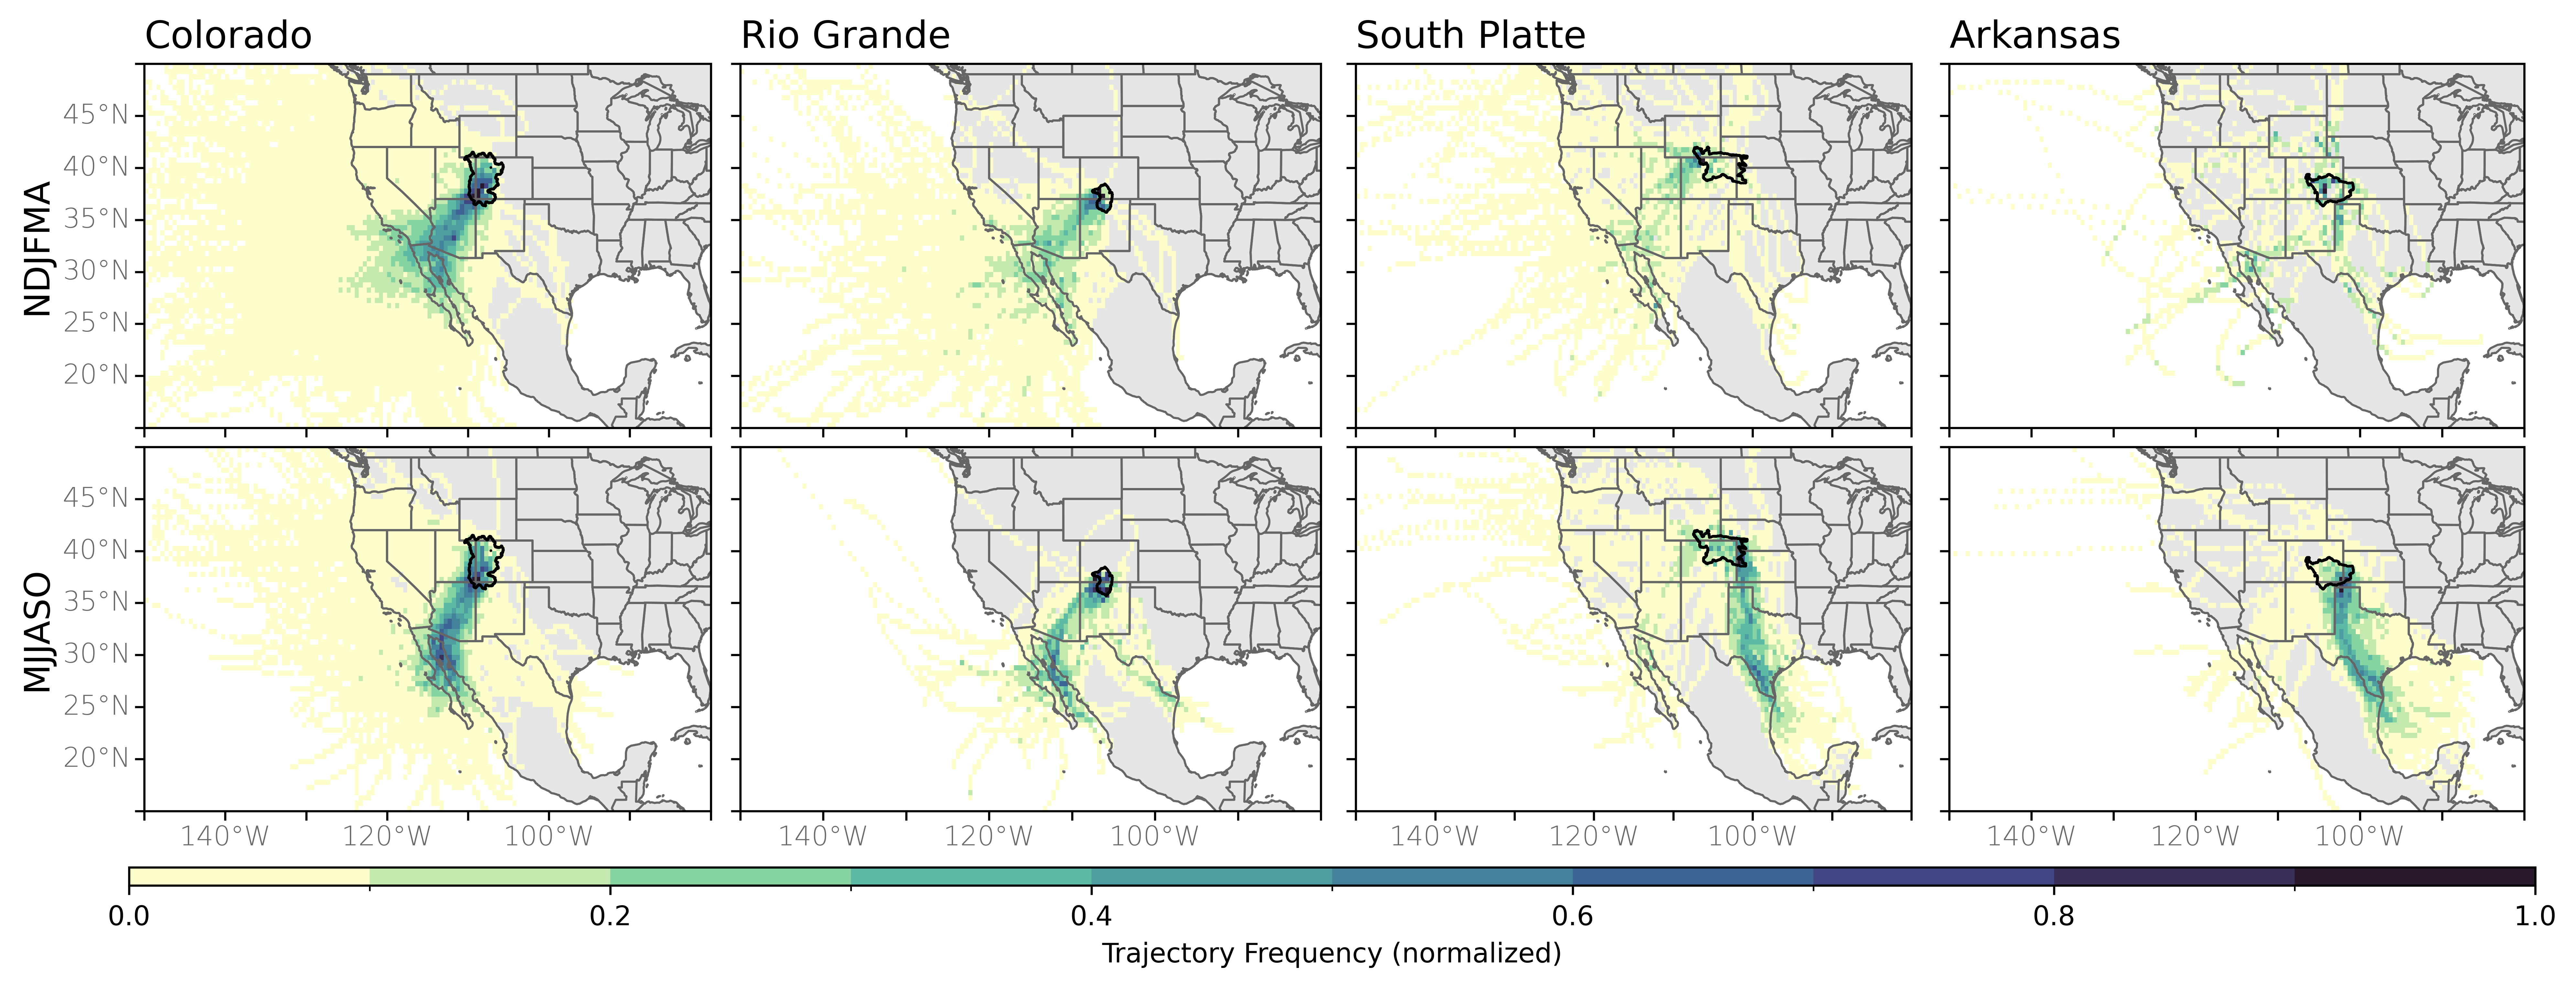
\includegraphics[width=\textwidth]{fig6.png}
\label{fig:heatmaps}
\caption{(a) The trajectory frequency (shading; \# normalized using the min-max method) for all Colorado subbasins that fall within the Colorado region (black contour) for the months of November to April from 2000 to 2023. (b) Same as (a) but for the Rio Grande region. (c) Same as (a) but for the South Platte region. (d) Same as (a) but for the Arkansas region. (e) Same as (a) but for the months of May to October. (f) Same as (e) but for the Rio Grande region. (g) Same as (e) but for the South Platte region. (h) Same as (e) but for the Arkansas region.}
\end{figure}

\subsection{Horizontal and Vertical Composites for Inland Penetrating ARs}
\label{sec:results:composite_analysis}

Synoptic conditions associated with Colorado inland-penetrating ARs were characterized by performing composites of daily mean (Fig. \ref{fig:composites_NDJFMA}a,d,g and \ref{fig:composites_MJJASO}a,d,g) and anomalies (annual cycle removed) (Fig. \ref{fig:anom_composites_NDJFMA}a,d,g and \ref{fig:anom_composites_MJJASO}a,d,g) for IVT (kg m\textsuperscript{-1} s\textsuperscript{-1}) and 700 hPa geopotential heights (m). The composites are broken down for cool and warm seasons and dates are chosen for each composite if any of the trajectories for any of the subbasins in Colorado were associated with an AR at the coast and passed through the indicated red bounding box in each figure. The bounding boxes were chosen based on the high frequency of trajectories identified in Fig. \ref{fig:heatmaps}. 

Mesoscale conditions associated with Colorado inland-penetrating ARs were characterized by performing composites of vertical cross-sections of daily mean (Fig. \ref{fig:composites_NDJFMA}b,c,e,f,h,i and \ref{fig:composites_MJJASO}b,c,e,f,h,i) and anomalies (annual cycle removed) (Fig. \ref{fig:anom_composites_NDJFMA}b,c,e,f,h,i and \ref{fig:anom_composites_MJJASO}b,c,e,f,h,i) for water vapor flux (m s\textsuperscript{-1}), freezing level (hPa), and trajectory frequency. To capture the moisture flux before and after potential topography, we show two cross-sections per region (see blue lines in Figs. \ref{fig:composites_NDJFMA}, \ref{fig:composites_MJJASO}, \ref{fig:anom_composites_NDJFMA}, and \ref{fig:anom_composites_MJJASO}). The dates for the vertical cross-section composites are chosen when any of the trajectories for any of the subbasins in Colorad were associated with an AR at the coast and passed through the indicated line. 

\begin{figure}
\noindent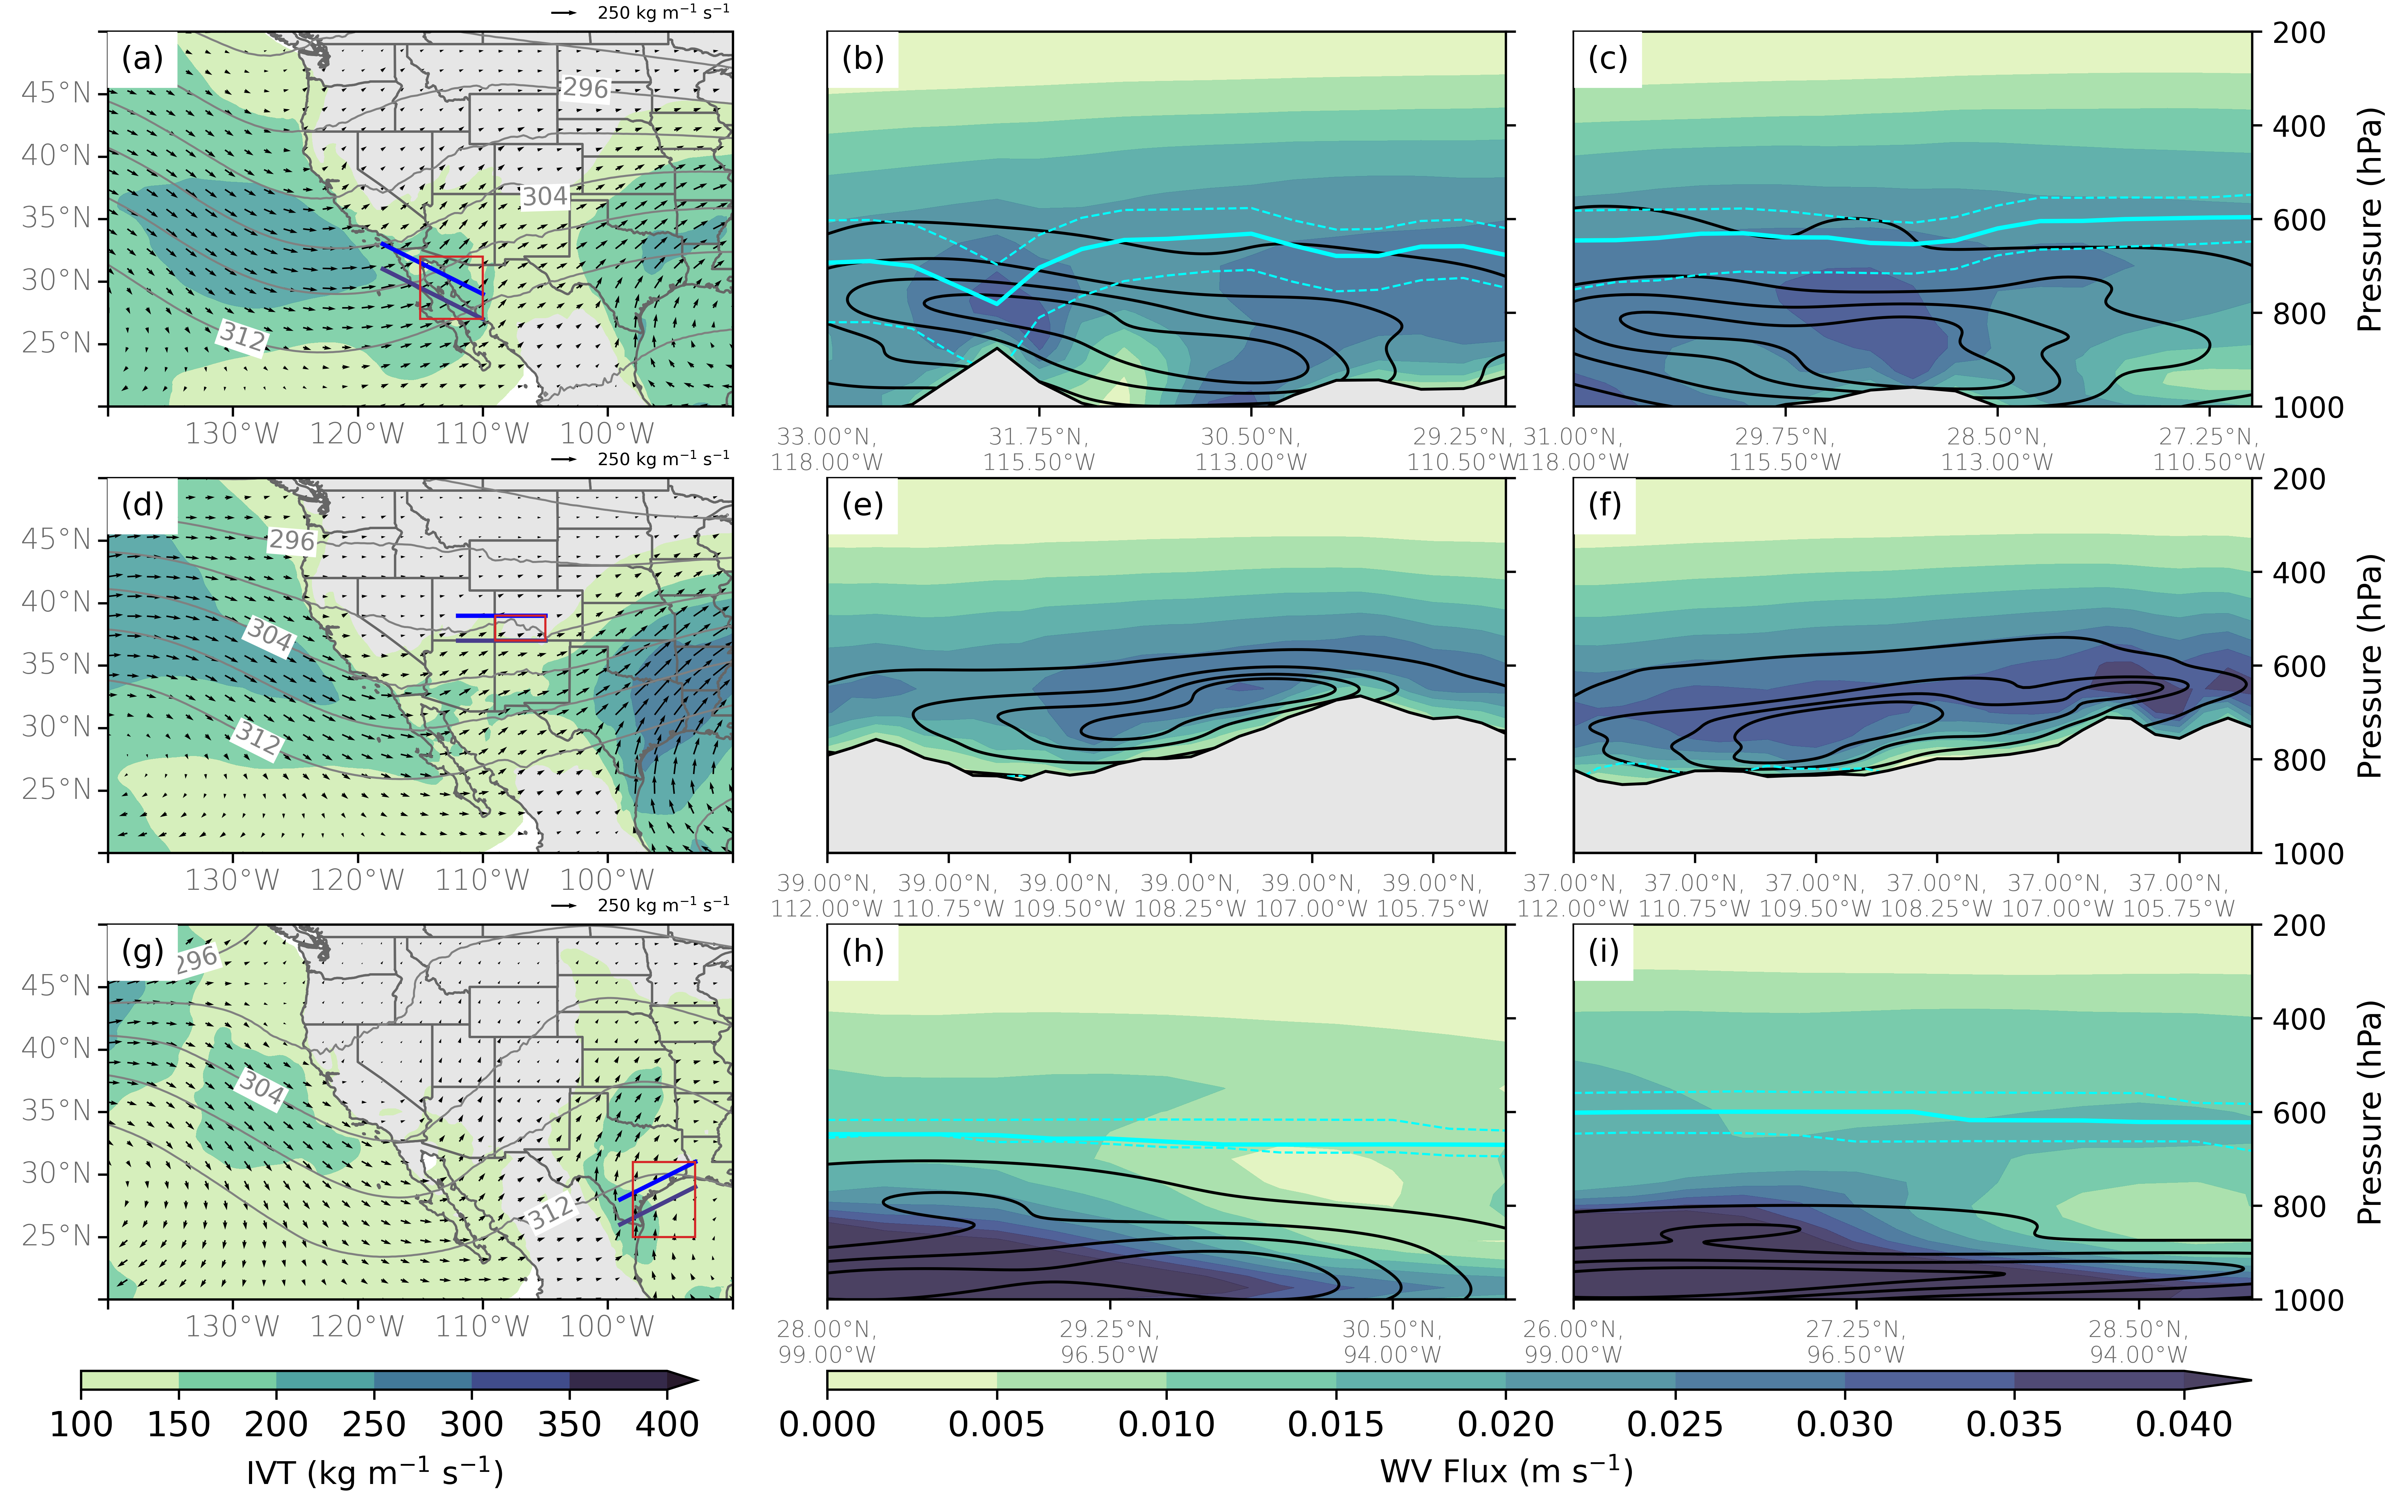
\includegraphics[width=\textwidth]{fig7.png}
\label{fig:composites_NDJFMA}
\caption{}
\end{figure}

\begin{figure}
\noindent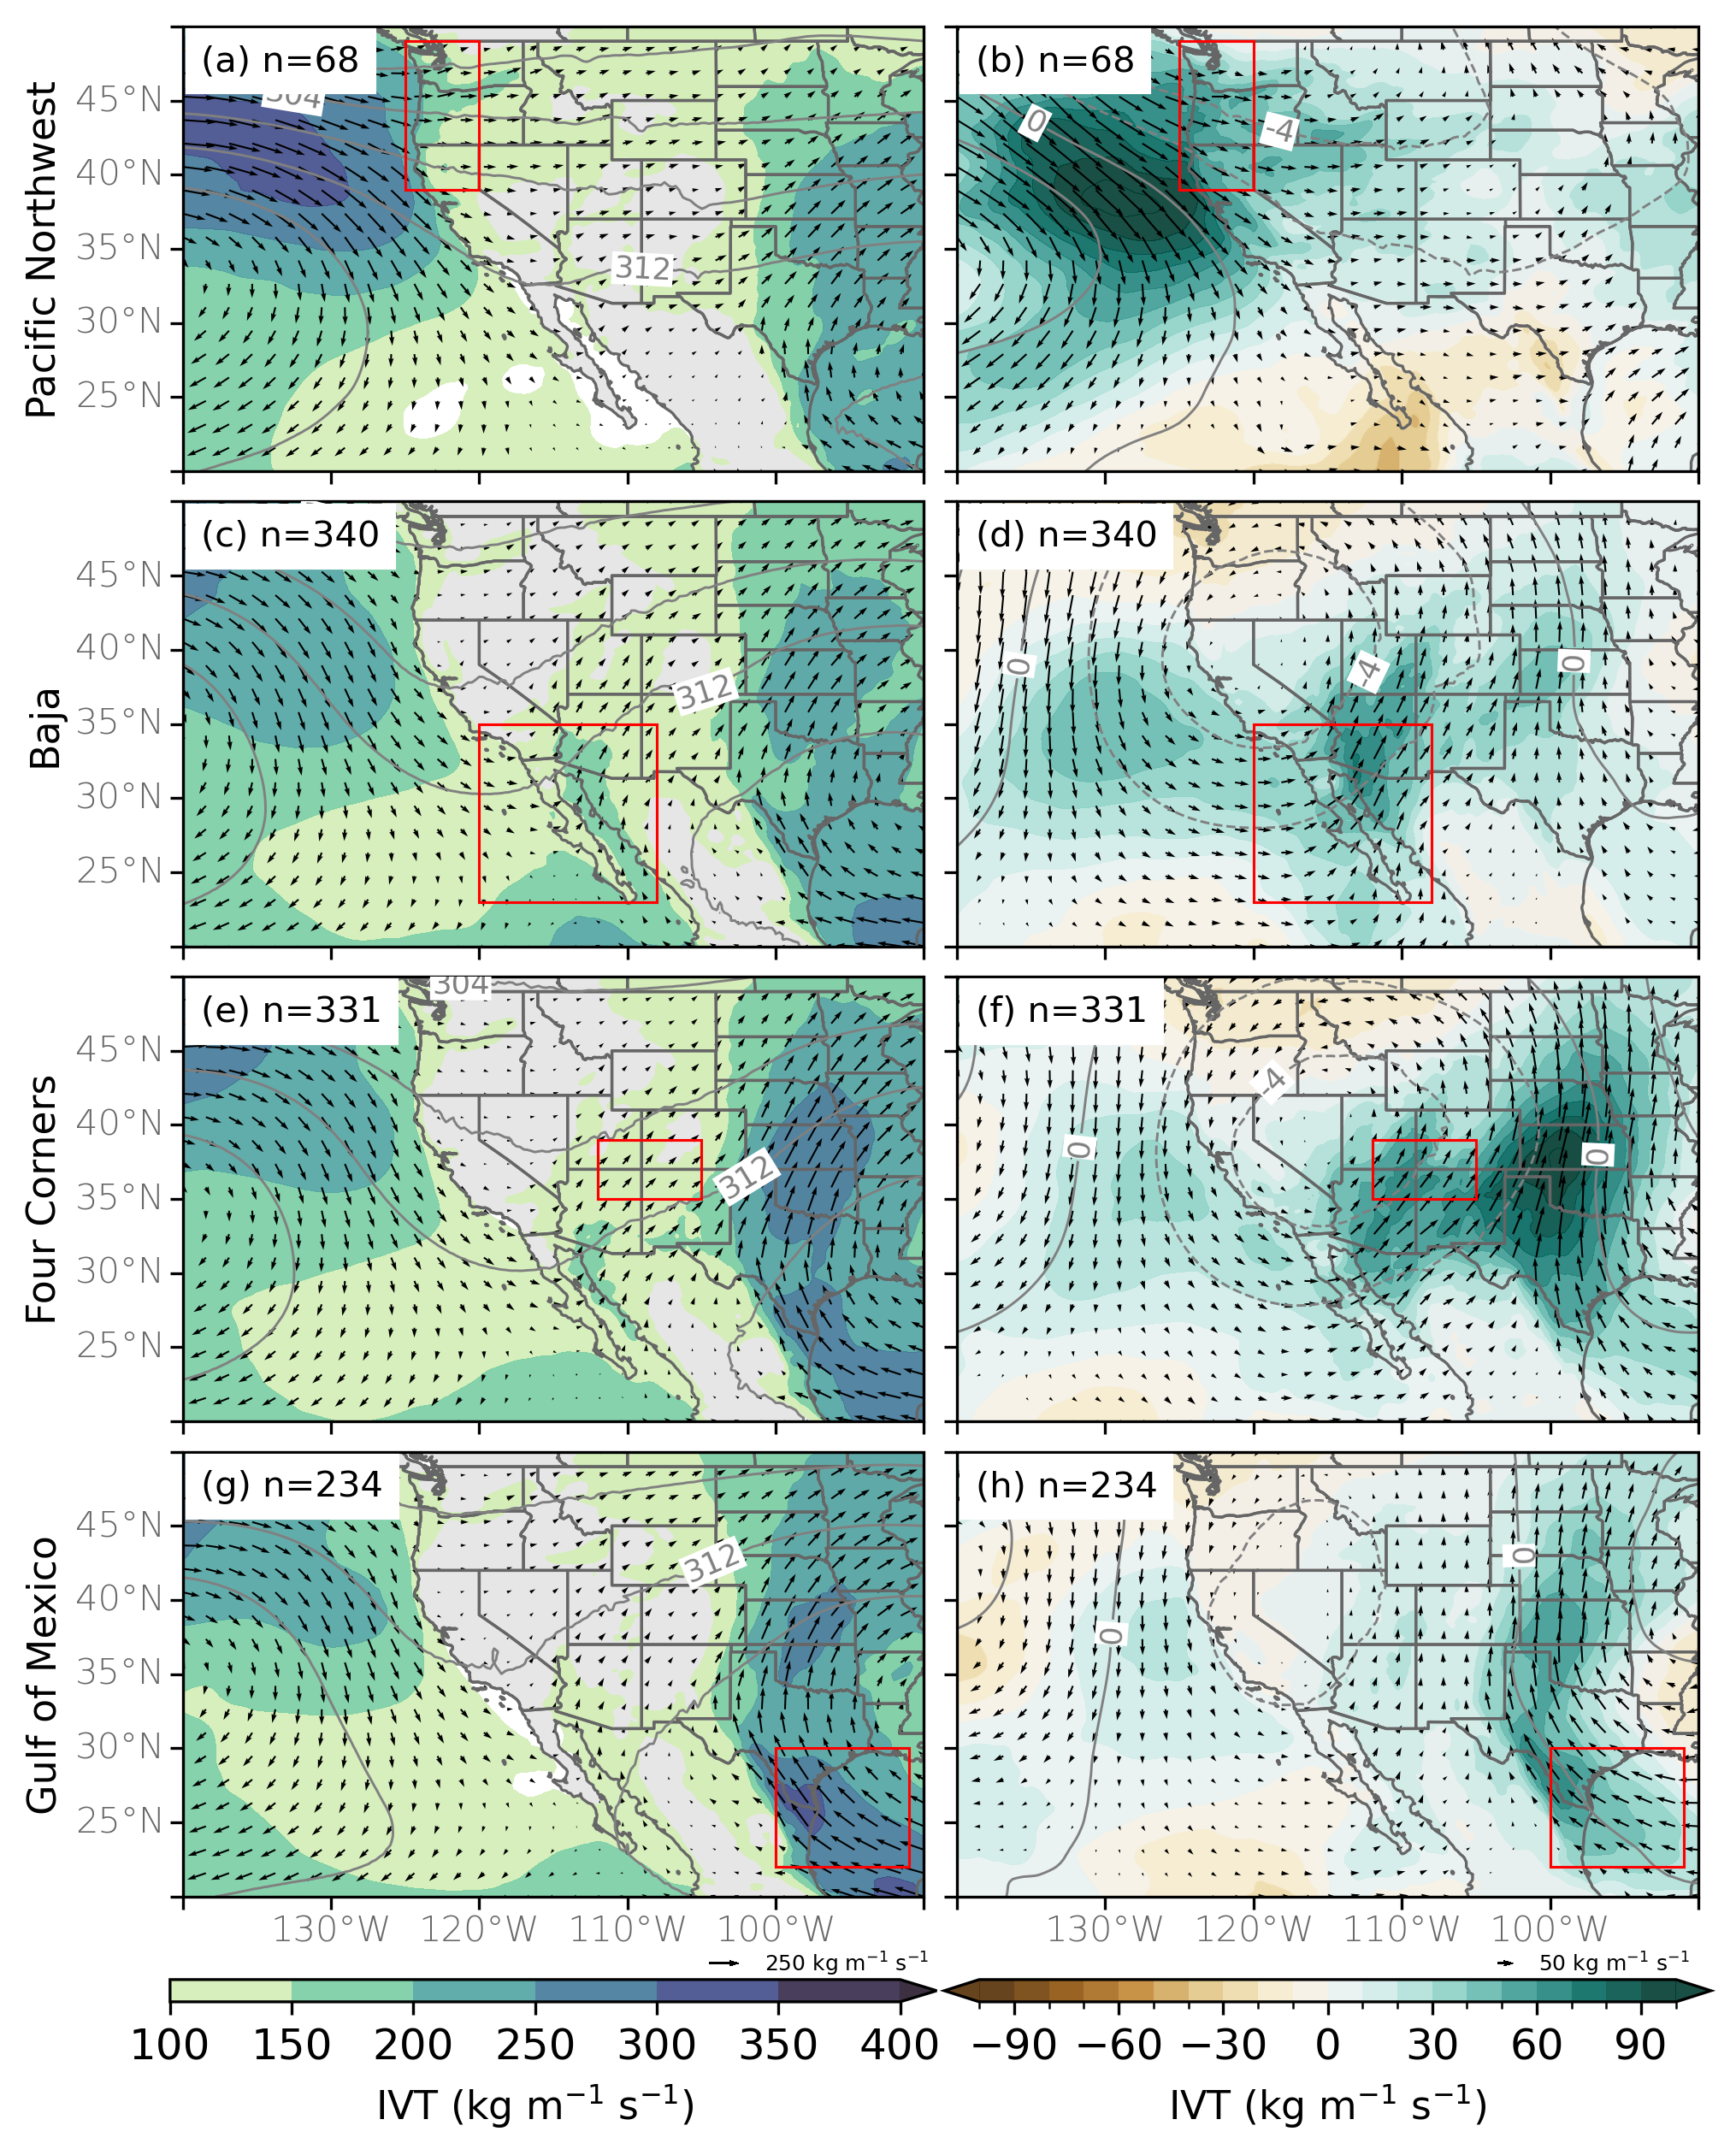
\includegraphics[width=\textwidth]{fig8.png}
\label{fig:composites_MJJASO}
\caption{}
\end{figure}

\begin{figure}
\noindent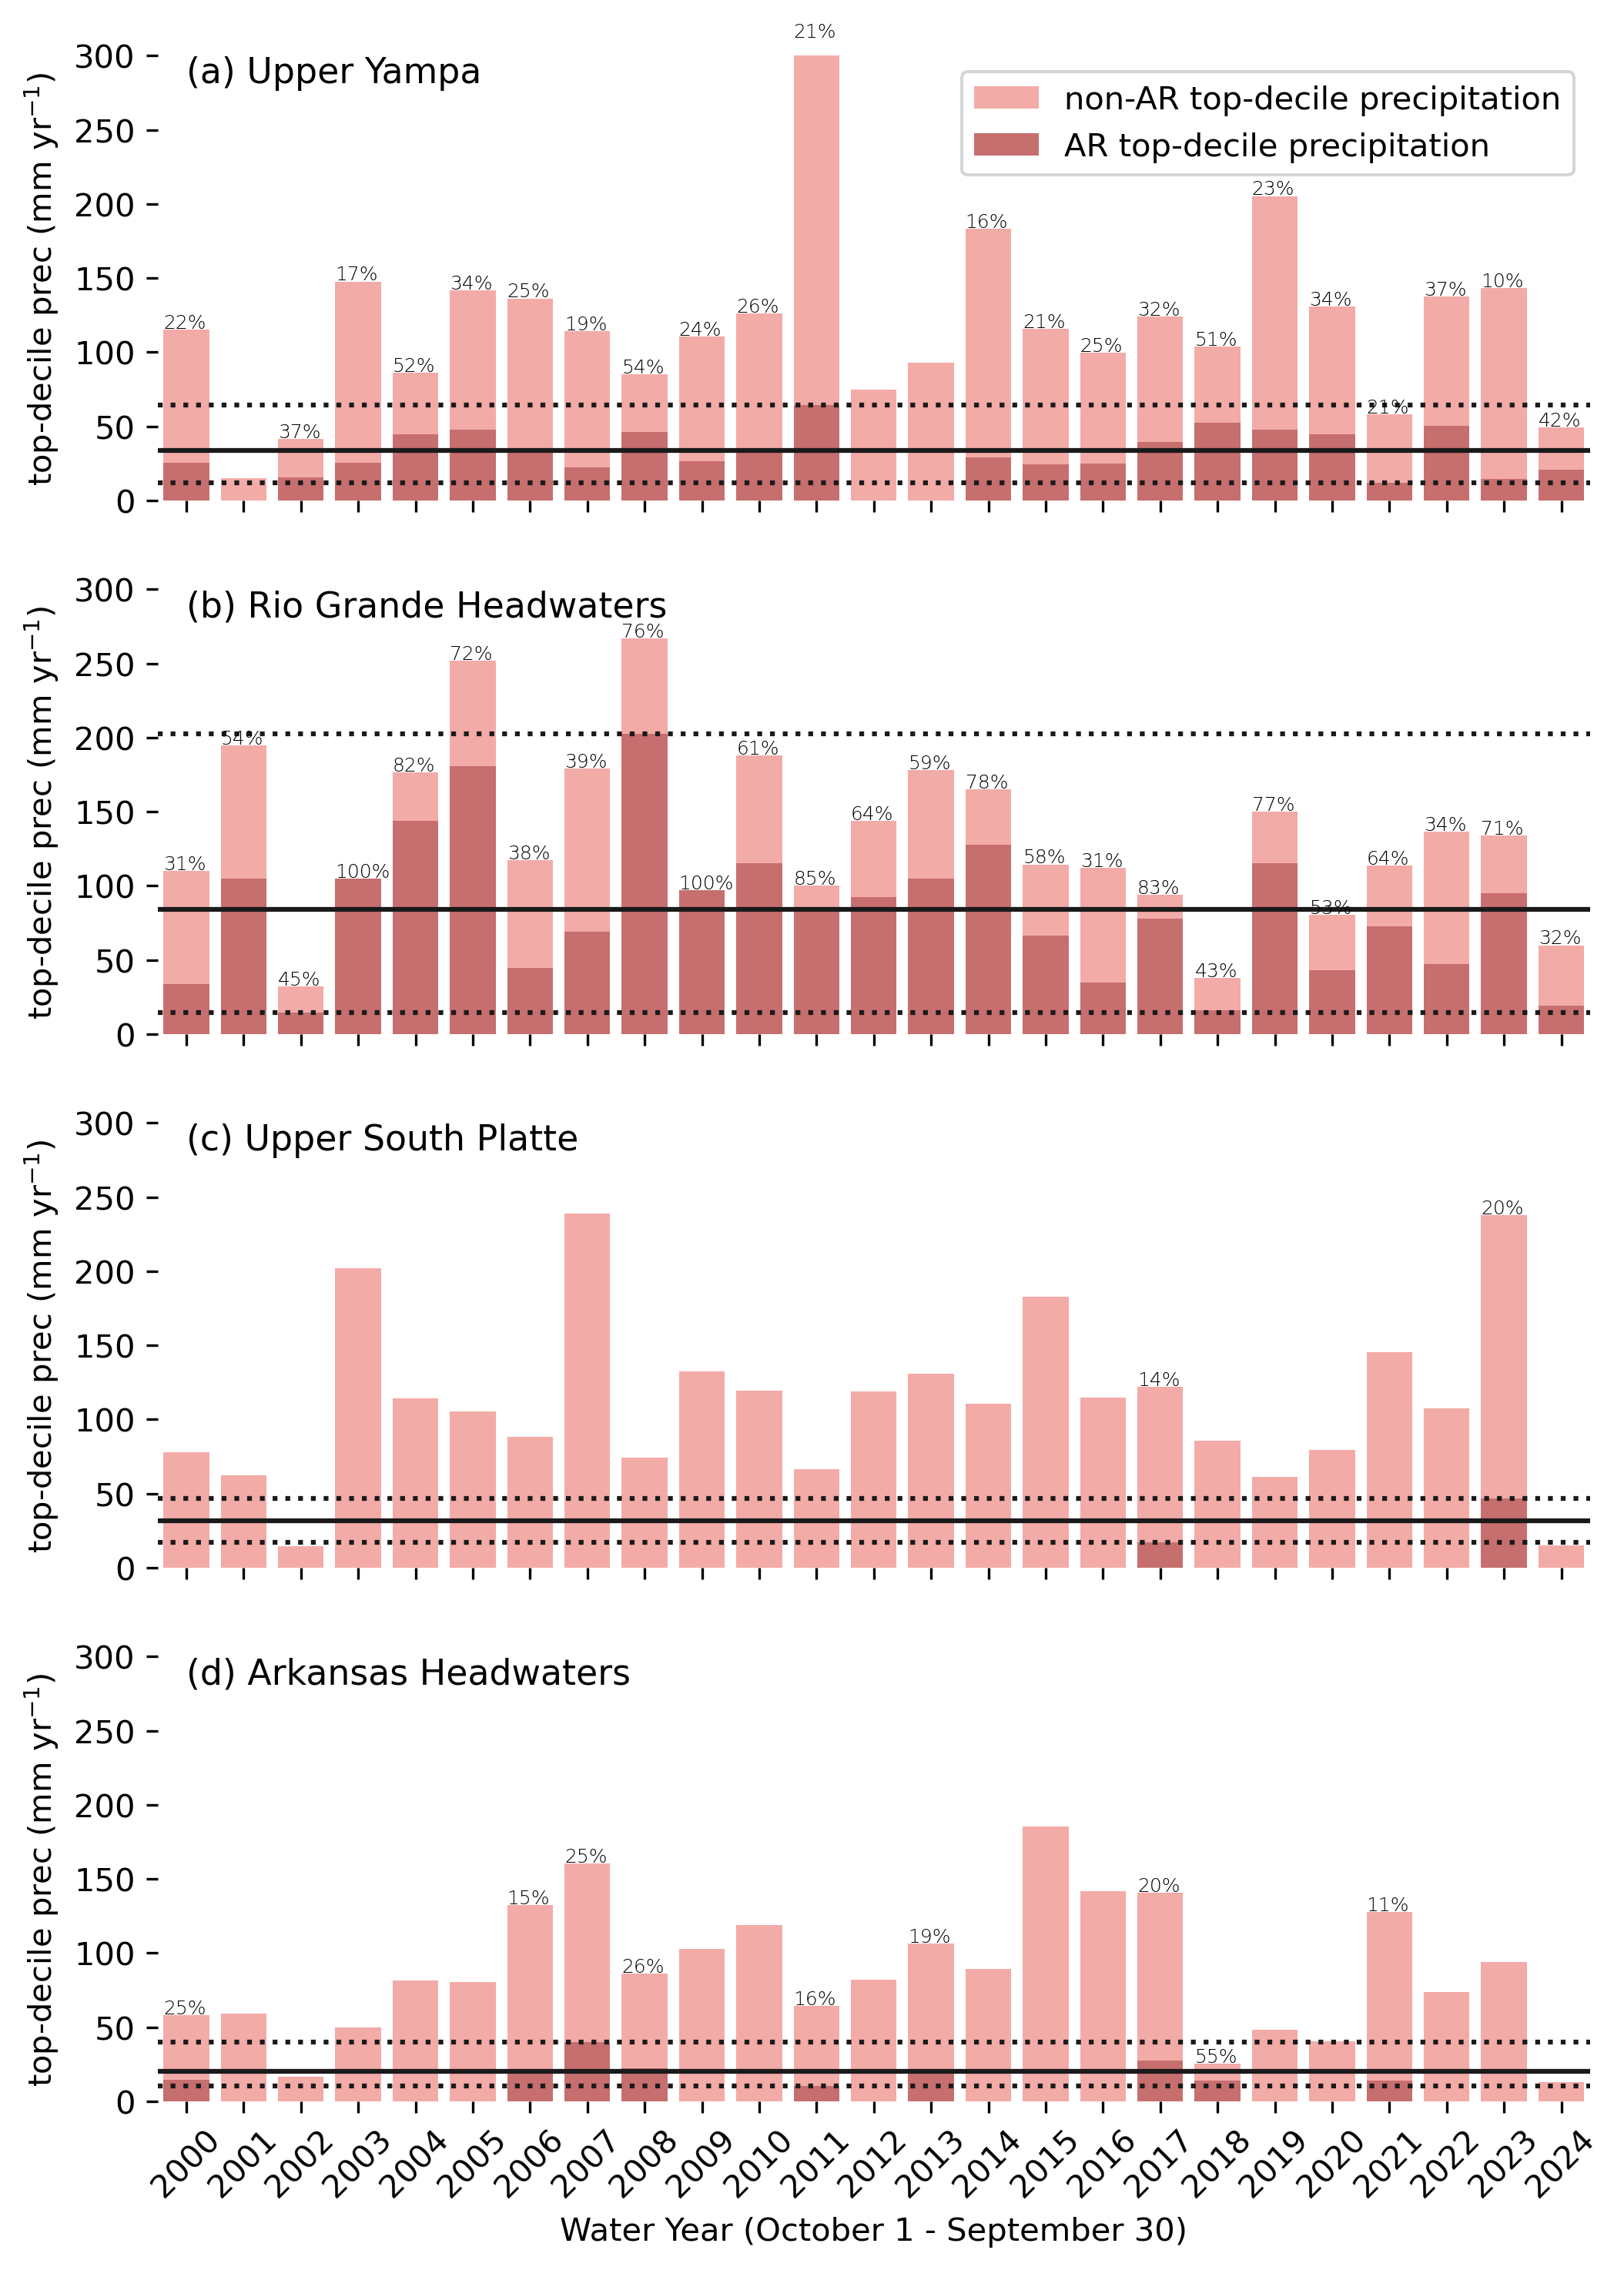
\includegraphics[width=\textwidth]{fig9.png}
\label{fig:anom_composites_NDJFMA}
\caption{}
\end{figure}

\begin{figure}
\noindent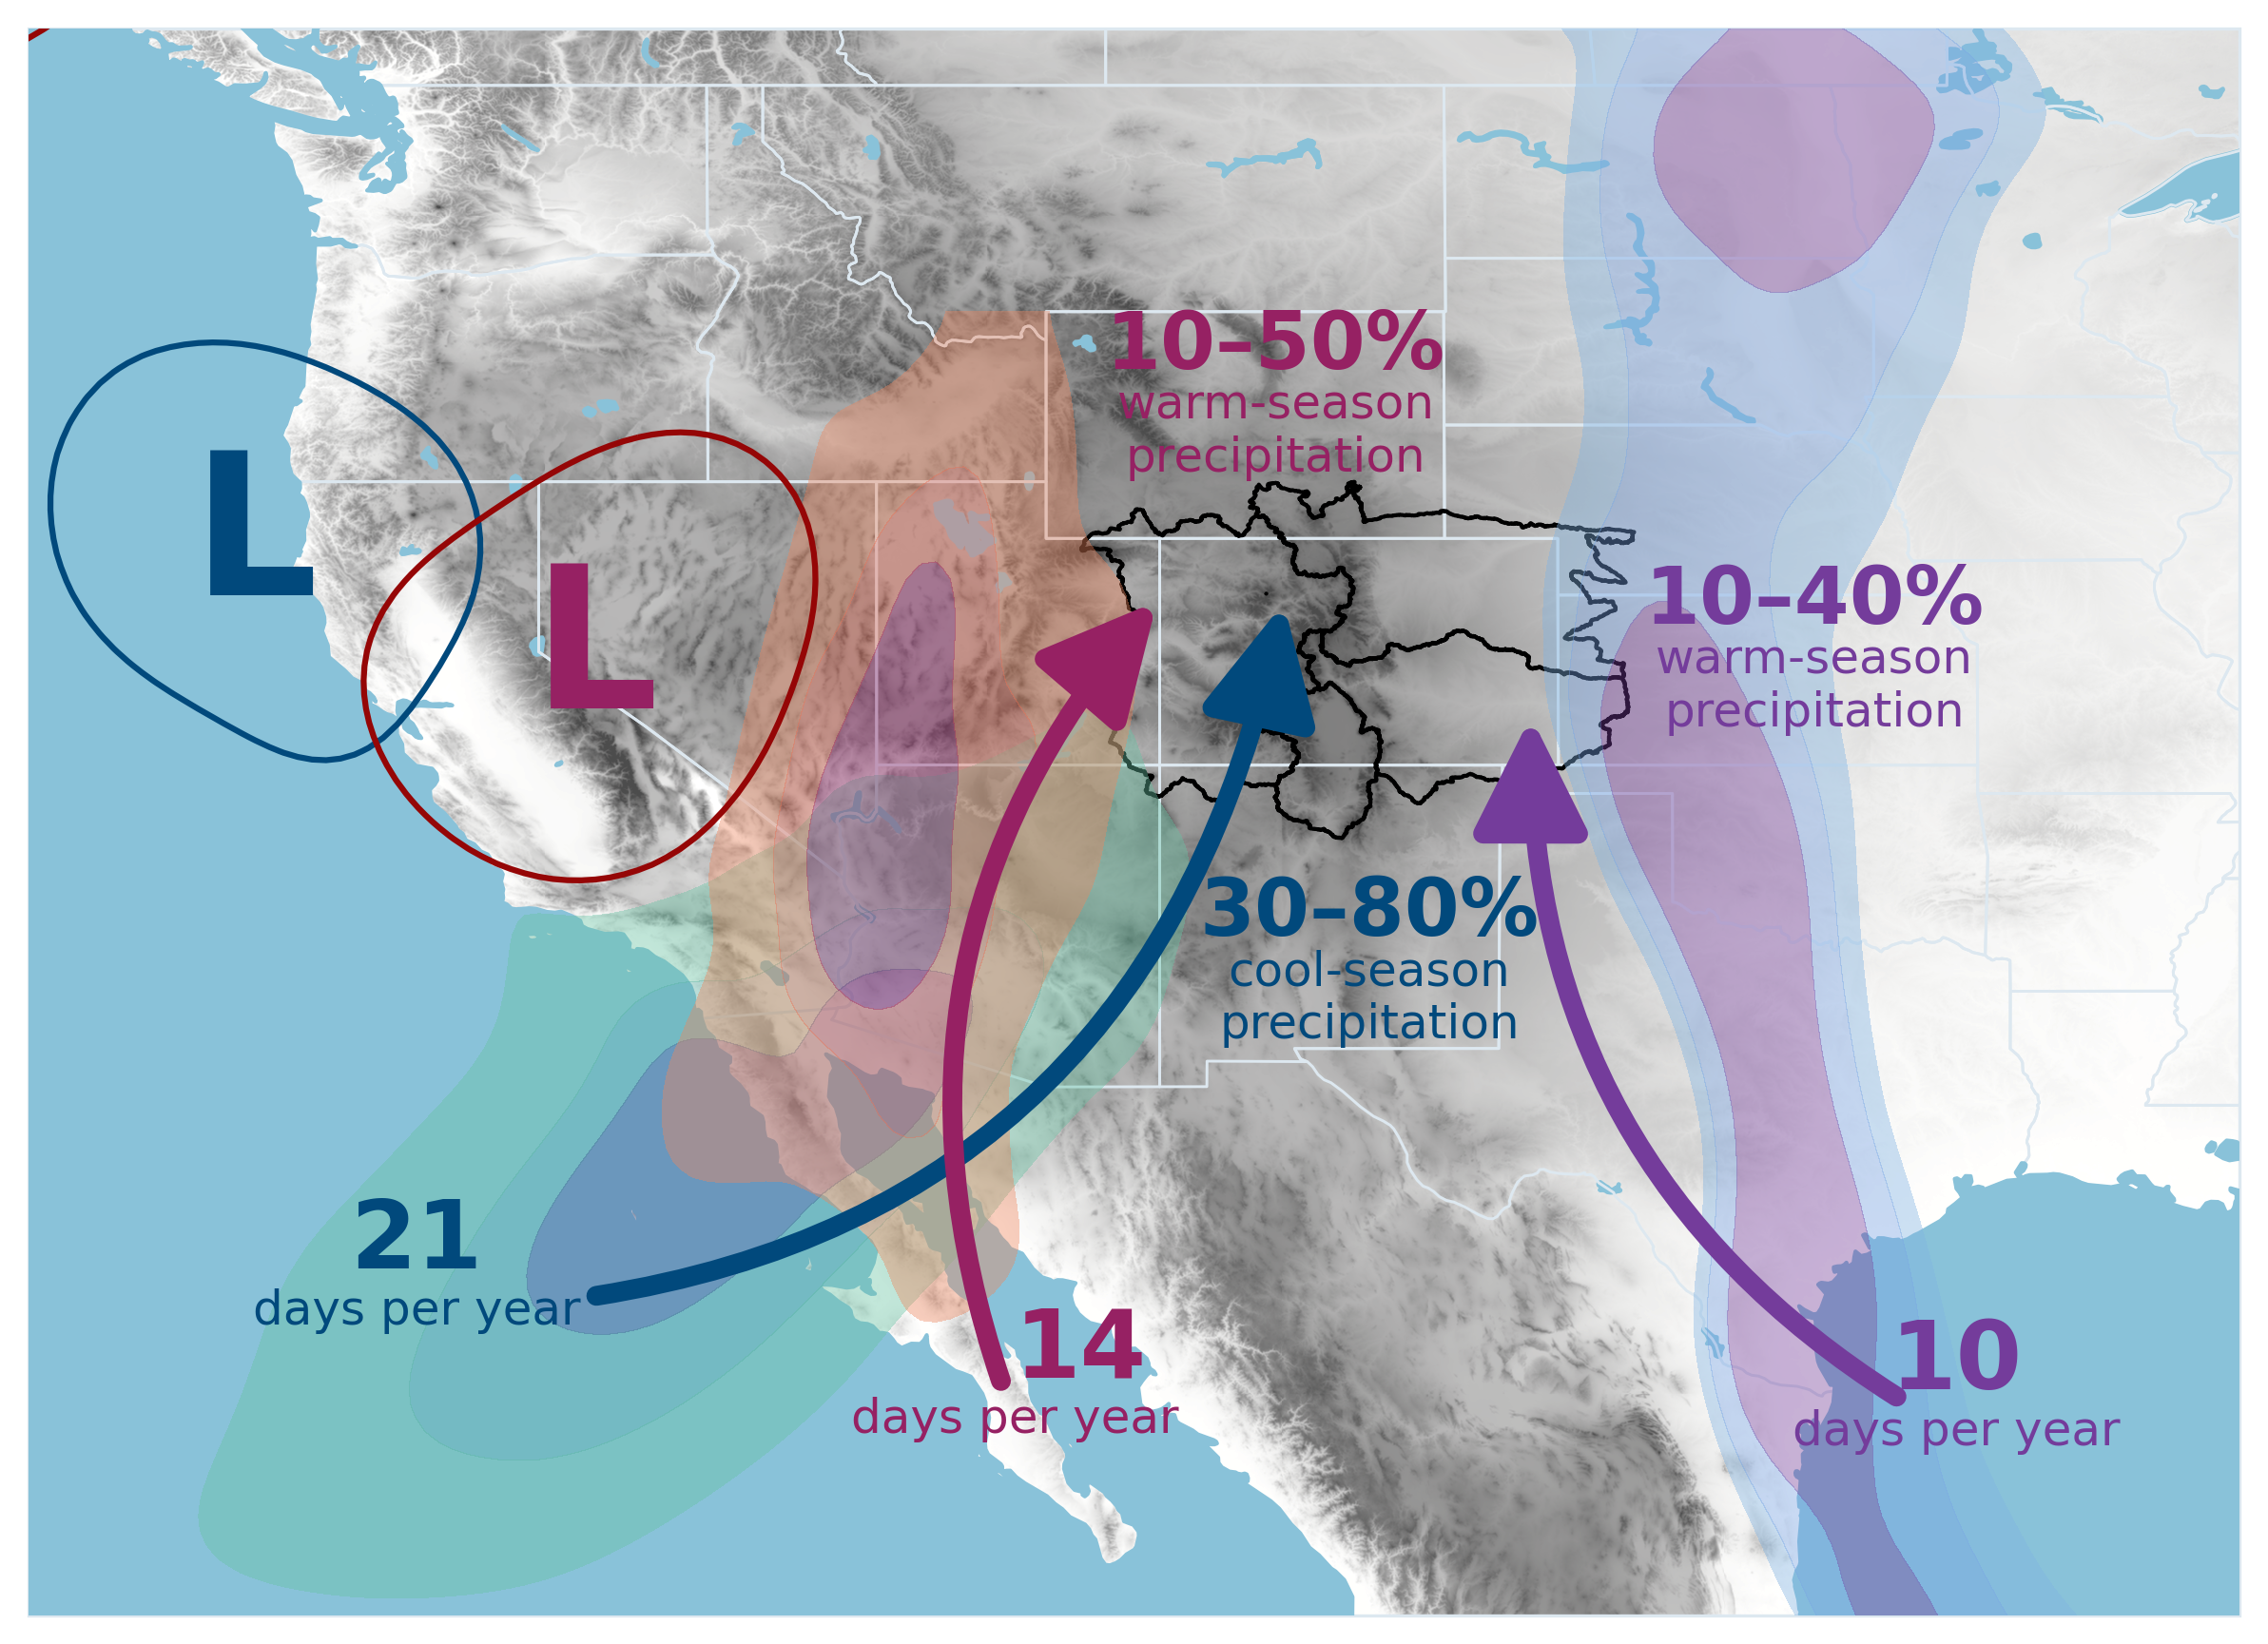
\includegraphics[width=\textwidth]{fig10.png}
\label{fig:anom_composites_MJJASO}
\caption{}
\end{figure}




\section{Conclusions}
\label{conclusions}
% Main Idea: This section will summarize the findings of the frequency, intensity, seasonality, and pathways of the inland penetrating moisture associated with Atmospheric Rivers and top-decile precipitation across Colorado.
% Introduce: Figure 8 will be a schematic similar to Rutz et al., 2015 (Figure 16 I think) that shows the common pathways and some associated statistics. 
% Key Point: This will summarize the findings of this paper.
% Explain Key Point: This key point will need to be made because it is the end of the paper.
% Connect: This will give a general understanding of the key findings of this work as well as provide a base for future directions (i.e., what questions were left unanswered)

% \section{= enter section title =}
%Text here ===>>>


%%

%  Numbered lines in equations:
%  To add line numbers to lines in equations,
%  \begin{linenomath*}
%  \begin{equation}
%  \end{equation}
%  \end{linenomath*}



%% Enter Figures and Tables near as possible to where they are first mentioned:
%
% DO NOT USE \psfrag or \subfigure commands.
%
% Figure captions go below the figure.
% Acronyms used in figure captions will be spelled out in the final, published version.

% Table titles go above tables;  other caption information
%  should be placed in last line of the table, using
% \multicolumn2l{$^a$ This is a table note.}
% NOTE that there is no difference between table caption and table heading in the final, published version
%
%----------------
% EXAMPLE FIGURES
%
% \begin{figure}
% 
\includegraphics{example.png}
% \caption{caption}
% \end{figure}
%
% Giving latex a width will help it to scale the figure properly. A simple trick is to use \textwidth. Try this if large figures run off the side of the page.
% \begin{figure}
% \noindent\includegraphics[width=\textwidth]{anothersample.png}
%\caption{caption}
%\label{pngfiguresample}
%\end{figure}
%
%
% If you get an error about an unknown bounding box, try specifying the width and height of the figure with the natwidth and natheight options. This is common when trying to add a PDF figure without pdflatex.
% \begin{figure}
% \noindent\includegraphics[natwidth=800px,natheight=600px]{samplefigure.pdf}
%\caption{caption}
%\label{pdffiguresample}
%\end{figure}
%
%
% PDFLatex does not seem to be able to process EPS figures. You may want to try the epstopdf package.
%

%
% ---------------
% EXAMPLE TABLE
%
% \begin{table}
% \caption{Time of the Transition Between Phase 1 and Phase 2$^{a}$}
% \centering
% \begin{tabular}{l c}
% \hline
%  Run  & Time (min)  \\
% \hline
%   $l1$  & 260   \\
%   $l2$  & 300   \\
%   $l3$  & 340   \\
%   $h1$  & 270   \\
%   $h2$  & 250   \\
%   $h3$  & 380   \\
%   $r1$  & 370   \\
%   $r2$  & 390   \\
% \hline
% \multicolumn{2}{l}{$^{a}$Footnote text here.}
% \end{tabular}
% \end{table}

%%%%%%%%%%%%%%%%%%%%%%%%%%%%%%%%%%%%%%%%%%%%%%%
% SIDEWAYS FIGURES and TABLES
% AGU prefers the use of {sidewaystable} over {landscapetable} as it causes fewer problems.
%
% \begin{sidewaysfigure}
% \includegraphics[width=20pc]{figsamp}
% \caption{caption here}
% \label{newfig}
% \end{sidewaysfigure}
%
%  \begin{sidewaystable}
%  \caption{Caption here}
% \label{tab:signif_gap_clos}
%  \begin{tabular}{ccc}
% one&two&three\\
% four&five&six
%  \end{tabular}
%  \end{sidewaystable}

%% If using numbered lines, please surround equations with \begin{linenomath*}...\end{linenomath*}
%\begin{linenomath*}
%\begin{equation}
%y|{f} \sim g(m, \sigma),
%\end{equation}
%\end{linenomath*}

%%% End of body of article

%%%%%%%%%%%%%%%%%%%%%%%%%%%%%%%%%%%%%%%%%%%%%%%
%% Optional Appendices go here
%
% The \appendix command resets counters and redefines section heads
%
% After typing \appendix
%
%\section{Here Is Appendix Title}
% will show
% A: Here Is Appendix Title
%
\appendix
\section{Calculation of IVT}    %% Appendix A
\label{appendix:ivt}
Integrated water vapor transport (IVT), a variable widely used for the detection and identification of ARs (e.g., \citeA{Guan2015, MartinRalph2019}) is calculated by taking the 3-hourly model data, interpolating u and v wind components (m s\textsuperscript{-1}), and water vapor mixing ratio (kg kg\textsuperscript{-1}) to 20 pressure levels (1000, 975, 950, 925, 900, 875, 850, 825, 800, 775, 750, 700, 650, 600, 550, 500, 450, 400, 350, and 300 hPa). Only data at pressure levels above ground level were used for each grid cell in the integration. Then, using water vapor mixing ratio, we computed specific humidity (q) and then integrated u and v wind components with q at all pressure levels above ground level using the following equations:

\begin{equation}
IVT_{x} = -\frac{1}{g} \int_{1000}^{300} u q dp
\end{equation}

\begin{equation}
IVT_{y} = -\frac{1}{g} \int_{1000}^{300} v q dp
\end{equation}

where g is the gravitational acceleration (m s\textsuperscript{-2}), u is zonal wind (m s\textsuperscript{-1}), v is meridional wind (m s\textsuperscript{-1}), q is specific humidity (kg kg\textsuperscript{-1}), p is pressure (Pa = kg m\textsuperscript{-1} s\textsuperscript{-2}), and the column integration is between pressure levels 1000 and 250 hPa inclusive.

The magnitude of IVT is calculated using the following equation:

\begin{equation}
IVT = \sqrt{IVT_{x}^2 + IVT_{y}^2}
\end{equation}

Specific humidity (kg kg \textsuperscript{-1}) is derived from water vapor mixing ratio (kg kg \textsuperscript{-1}) using the formula from \cite{Wallace2006} where q is specific humidity and w is the water vapor mixing ratio.

\begin{equation}
q = \frac{w}{1 + w}
\end{equation}

\section{Calculation of Water Vapor Flux}    %% Appendix B
\label{appendix:wvf}
Water vapor flux, a variable used in multiple AR-related studies to examine the vertical profile of water vapor (e.g., \citeA{Guan2015}), is the flux of water vapor at each identified pressure level. The following equations were used to calculate water vapor flux: 

\begin{equation}
VT_{u}^{p}   = q*u 
\end{equation}
\begin{equation}
VT_{v}^{p}   = q*v   
\end{equation}
\begin{equation}
VT = \sqrt{VT^{2}_{u} + VT^{2}_{v}}
\end{equation}

where q is specific humidity (kg kg\textsuperscript{-1}), u is zonal wind (m s\textsuperscript{-1}), v is meridional wind (m s\textsuperscript{-1}) at specified pressure, p. If specific humidity retains its kg kg\textsuperscript{-1}, the resulting units for water vapor flux are m s\textsuperscript{-1}. 

%%%%%%%%%%%%%%%%%%%%%%%%%%%%%%%%%%%%%%%%%%%%%%%
% Optional Glossary, Notation or Acronym section goes here:
%
% Glossary is only allowed in Reviews of Geophysics
%  \begin{glossary}
%  \term{Term}
%   Term Definition here
%  \term{Term}
%   Term Definition here
%  \term{Term}
%   Term Definition here
%  \end{glossary}


%%%%%%%%%%%%%%%%%%%%%%%%%%%%%%%%%%%%%%%%%%%%%%%
% Acronyms
%% NOTE that acronyms in the final published version will be spelled out when used in figure captions.
%   \begin{acronyms}
%   \acro{Acronym}
%   Definition here
%   \acro{EMOS}
%   Ensemble model output statistics
%   \acro{ECMWF}
%   Centre for Medium-Range Weather Forecasts
%   \end{acronyms}


%%%%%%%%%%%%%%%%%%%%%%%%%%%%%%%%%%%%%%%%%%%%%%%
% Notation
%   \begin{notation}
%   \notation{$a+b$} Notation Definition here
%   \notation{$e=mc^2$}
%   Equation in German-born physicist Albert Einstein's theory of special
%  relativity that showed that the increased relativistic mass ($m$) of a
%  body comes from the energy of motion of the body—that is, its kinetic
%  energy ($E$)—divided by the speed of light squared ($c^2$).
%   \end{notation}




%%%%%%%%%%%%%%%%%%%%%%%%%%%%%%%%%%%%%%%%%%%%%%%
%
% DATA SECTION and ACKNOWLEDGMENTS
%
%%%%%%%%%%%%%%%%%%%%%%%%%%%%%%%%%%%%%%%%%%%%%%%

\section*{Open Research Section}
This section MUST contain a statement that describes where the data supporting the conclusions can be obtained. Data cannot be listed as ''Available from authors'' or stored solely in supporting information. Citations to archived data should be included in your reference list. Wiley will publish it as a separate section on the paper’s page. Examples and complete information are here:
https://www.agu.org/Publish with AGU/Publish/Author Resources/Data for Authors

PRISM Climate Group, Oregon State University, https://prism.oregonstate.edu, data created 4 Feb 2014, accessed 16 Dec 2020.

Download the Colorado Watershed Boundary Dataset (WBD) Hydrologic Unit 8
The shapefile is available for download from https://geo.colorado.edu/catalog/47540-5c8ff914a84a6c000a68f3a8.


\acknowledgments
Enter acknowledgments here. This section is to acknowledge funding, thank colleagues, enter any secondary affiliations, and so on.


%%%%%%%%%%%%%%%%%%%%%%%%%%%%%%%%%%%%%%%%%%%%%%%
% REFERENCES and BIBLIOGRAPHY
%
% \bibliography{<name of your .bib file>} don't specify the file extension
% don't specify bibliographystyle
%
%%%%%%%%%%%%%%%%%%%%%%%%%%%%%%%%%%%%%%%%%%%%%%%

\bibliography{references}



%Reference citation instructions and examples:
%
% Please use ONLY \cite and \citeA for reference citations.
% \cite for parenthetical references
% ...as shown in recent studies (Simpson et al., 2019)
% \citeA for in-text citations
% ...Simpson et al. (2019) have shown...
%
%
%...as shown by \citeA{jskilby}.
%...as shown by \citeA{lewin76}, \citeA{carson86}, \citeA{bartoldy02}, and \citeA{rinaldi03}.
%...has been shown \cite{jskilbye}.
%...has been shown \cite{lewin76,carson86,bartoldy02,rinaldi03}.
%... \cite <i.e.>[]{lewin76,carson86,bartoldy02,rinaldi03}.
%...has been shown by \cite <e.g.,>[and others]{lewin76}.
%
% apacite uses < > for prenotes and [ ] for postnotes
% DO NOT use other cite commands (e.g., \citet, \citep, \citeyear, \nocite, \citealp, etc.).
%



\end{document}



More Information and Advice:

%%%%%%%%%%%%%%%%%%%%%%%%%%%%%%%%%%%%%%%%%%%%%%%
%
%  SECTION HEADS
%
%%%%%%%%%%%%%%%%%%%%%%%%%%%%%%%%%%%%%%%%%%%%%%%

% Capitalize the first letter of each word (except for
% prepositions, conjunctions, and articles that are
% three or fewer letters).

% AGU follows standard outline style; therefore, there cannot be a section 1 without
% a section 2, or a section 2.3.1 without a section 2.3.2.
% Please make sure your section numbers are balanced.
% ---------------
% Level 1 head
%
% Use the \section{} command to identify level 1 heads;
% type the appropriate head wording between the curly
% brackets, as shown below.
%
%An example:
%\section{Level 1 Head: Introduction}
%
% ---------------
% Level 2 head
%
% Use the \subsection{} command to identify level 2 heads.
%An example:
%\subsection{Level 2 Head}
%
% ---------------
% Level 3 head
%
% Use the \subsubsection{} command to identify level 3 heads
%An example:
%\subsubsection{Level 3 Head}
%
%---------------
% Level 4 head
%
% Use the \subsubsubsection{} command to identify level 3 heads
% An example:
%\subsubsubsection{Level 4 Head} An example.
%
%%%%%%%%%%%%%%%%%%%%%%%%%%%%%%%%%%%%%%%%%%%%%%%
%
%  IN-TEXT LISTS
%
%%%%%%%%%%%%%%%%%%%%%%%%%%%%%%%%%%%%%%%%%%%%%%%
%
% Do not use bulleted lists; enumerated lists are okay.
% \begin{enumerate}
% \item
% \item
% \item
% \end{enumerate}
%
%%%%%%%%%%%%%%%%%%%%%%%%%%%%%%%%%%%%%%%%%%%%%%%
%
%  EQUATIONS
%
%%%%%%%%%%%%%%%%%%%%%%%%%%%%%%%%%%%%%%%%%%%%%%%

% Single-line equations are centered.
% Equation arrays will appear left-aligned.

Math coded inside display math mode \[ ...\]
 will not be numbered, e.g.,:
 \[ x^2=y^2 + z^2\]

 Math coded inside \begin{equation} and \end{equation} will
 be automatically numbered, e.g.,:
 \begin{equation}
 x^2=y^2 + z^2
 \end{equation}


% To create multiline equations, use the
% \begin{eqnarray} and \end{eqnarray} environment
% as demonstrated below.
\begin{eqnarray}
  x_{1} & = & (x - x_{0}) \cos \Theta \nonumber \\
        && + (y - y_{0}) \sin \Theta  \nonumber \\
  y_{1} & = & -(x - x_{0}) \sin \Theta \nonumber \\
        && + (y - y_{0}) \cos \Theta.
\end{eqnarray}

%If you don't want an equation number, use the star form:
%\begin{eqnarray*}...\end{eqnarray*}

% Break each line at a sign of operation
% (+, -, etc.) if possible, with the sign of operation
% on the new line.

% Indent second and subsequent lines to align with
% the first character following the equal sign on the
% first line.

% Use an \hspace{} command to insert horizontal space
% into your equation if necessary. Place an appropriate
% unit of measure between the curly braces, e.g.
% \hspace{1in}; you may have to experiment to achieve
% the correct amount of space.


%%%%%%%%%%%%%%%%%%%%%%%%%%%%%%%%%%%%%%%%%%%%%%%
%
%  EQUATION NUMBERING: COUNTER
%
%%%%%%%%%%%%%%%%%%%%%%%%%%%%%%%%%%%%%%%%%%%%%%%

% You may change equation numbering by resetting
% the equation counter or by explicitly numbering
% an equation.

% To explicitly number an equation, type \eqnum{}
% (with the desired number between the brackets)
% after the \begin{equation} or \begin{eqnarray}
% command.  The \eqnum{} command will affect only
% the equation it appears with; LaTeX will number
% any equations appearing later in the manuscript
% according to the equation counter.
%

% If you have a multiline equation that needs only
% one equation number, use a \nonumber command in
% front of the double backslashes (\\) as shown in
% the multiline equation above.

% If you are using line numbers, remember to surround
% equations with \begin{linenomath*}...\end{linenomath*}

%  To add line numbers to lines in equations:
%  \begin{linenomath*}
%  \begin{equation}
%  \end{equation}
%  \end{linenomath*}



